% =====================================================================
% Artículo final — Taller 2 (Fases 2 y 3)
% Modelación de Ecuaciones Estructurales — Universidad Santo Tomás
% Compilar con: pdflatex articulo && bibtex articulo && pdflatex articulo && pdflatex articulo
% =====================================================================
\documentclass[11pt,a4paper]{article}

\usepackage[utf8]{inputenc}
\usepackage[T1]{fontenc}
\usepackage{lmodern}
\usepackage[spanish,es-tabla]{babel}
\usepackage[margin=2.5cm]{geometry}
\usepackage{booktabs}
\usepackage{longtable}
\usepackage{array}
\usepackage{multirow}
\usepackage{tabularx}
\usepackage{graphicx}
\usepackage{amsmath,amssymb}
\usepackage[round,authoryear]{natbib}
\usepackage[hidelinks]{hyperref}
\usepackage{caption}
\usepackage{float}
\usepackage{microtype}

\captionsetup{font=small,labelfont=bf}
\graphicspath{{figuras/}{salidas/}}
\setlength{\parskip}{0.4em}
\setlength{\parindent}{1.2em}

\newcommand{\chisq}{$\chi^2$}
\newcommand{\df}{\textit{gl}}

% =====================================================================
\begin{document}

\begin{center}
{\LARGE\bfseries Liderazgo, clima y satisfacción en el empleo público\\[2pt]
colombiano: un modelo de ecuaciones estructurales\\[2pt]
con indicadores ordinales\par}
\vspace{10pt}

{\large Kevin Leonardo Chaparro Reyes \quad Valentina Muñoz Palma \quad Paula Margarita Triana Ancinez\par}
\vspace{4pt}
{\normalsize Universidad Santo Tomás --- Facultad de Estadística\par}
{\normalsize Modelación de Ecuaciones Estructurales\par}
{\normalsize Docente: Juan Carlos Rubriche\par}
{\normalsize Bogotá D.C., Colombia\par}
\end{center}

\vspace{6pt}

% ---------------------------------------------------------------------
\section*{Resumen}
\addcontentsline{toc}{section}{Resumen}

Este artículo estima y evalúa un modelo de mediación parcial entre liderazgo directivo,
clima laboral y satisfacción laboral en el empleo público colombiano, con los microdatos
de la Encuesta sobre Ambiente y Desempeño Institucional (EDI 2025) del DANE. Se trabajó con
26.742 servidores públicos agrupados en 201 entidades y 19 indicadores ordinales. El modelo
de medición se estimó con mínimos cuadrados ponderados diagonalmente con media y varianza
ajustadas (WLSMV) y errores estándar robustos a la conglomeración por entidad; el modelo
estructural se contrastó con la prueba de diferencia escalada y los efectos indirectos se
evaluaron por simulación de Monte Carlo y por un bootstrap de 2.000 remuestras por
conglomerados. El análisis factorial confirmatorio final presentó un ajuste satisfactorio
(CFI = 0,988; TLI = 0,986; RMSEA = 0,050; SRMR = 0,025), aunque el RMSEA robusto asciende a
0,070, con cargas estandarizadas entre 0,623 y 0,931, fiabilidad compuesta superior a 0,89 y
AVE superior a 0,62. El modelo estructural reprodujo el ajuste del modelo de medición (ambos
con \chisq{} = 8.856,34 y 148 \df), de modo que la comparación entre ambos no es
informativa. Las cuatro hipótesis recibieron apoyo: liderazgo predice el clima
($\beta$ = 0,725), el clima predice la satisfacción ($\beta$ = 0,349) y el liderazgo
mantiene un efecto directo ($\beta$ = 0,447), con un efecto indirecto estandarizado de 0,230
(Monte Carlo) y 0,190 (bootstrap). La invarianza de medición se sostuvo por sexo y por sector
en los niveles configural, de umbrales, métrico y escalar. La evidencia es consistente con una
mediación parcial del clima, con implicaciones para la gestión del talento humano público.

\vspace{6pt}
\noindent\textbf{Palabras clave:} modelos de ecuaciones estructurales; liderazgo;
clima laboral; satisfacción laboral; invarianza de medición.

\vspace{10pt}
\section*{Abstract}
\addcontentsline{toc}{section}{Abstract}

This article estimates and evaluates a partial mediation model linking supervisory
leadership, work climate and job satisfaction in the Colombian public sector, using
microdata from the 2025 Survey on Institutional Environment and Performance (EDI) of DANE.
The sample comprises 26,742 public servants nested in 201 entities and 19 five-category
ordinal indicators. The measurement model was estimated with diagonally weighted least
squares with adjusted means and variances (WLSMV) and cluster-robust standard errors; the
structural model was tested with the scaled difference test, and indirect effects were
assessed through Monte Carlo simulation and a 2,000-replicate cluster bootstrap. The final
confirmatory factor model showed satisfactory fit (CFI = 0.988; TLI = 0.986;
RMSEA = 0.050; SRMR = 0.025), although the cluster-robust RMSEA rises to 0.070, with
standardized loadings between 0.623 and 0.931,
composite reliability between 0.892 and 0.973, and average variance extracted between
0.628 and 0.785. The structural model reproduced the fit of the measurement model (both
with \chisq{} = 8,856.34 and 148 \df), confirming that the structural block is saturated and
that the comparison between them is uninformative. All four hypotheses were supported:
leadership predicts climate ($\beta$ = 0.725), climate predicts satisfaction
($\beta$ = 0.349), and leadership retains a direct effect on satisfaction
($\beta$ = 0.447), with a standardized indirect effect of 0.230 (Monte Carlo) and 0.190
(cluster bootstrap). Measurement invariance held
across sex and sector at the configural, threshold, metric and scalar levels. The evidence is
consistent with a partial transmission of the leadership effect on satisfaction through
climate, with implications for human resource management in the public sector.

\vspace{6pt}
\noindent\textbf{Keywords:} structural equation modeling; leadership; work climate; job
satisfaction; measurement invariance.

\newpage

% =====================================================================
\section{Introducción}
% =====================================================================

La eficiencia, la legitimidad y la capacidad operativa del Estado dependen en buena medida
de la calidad del talento humano que integra el servicio público. En la administración
pública colombiana, el fortalecimiento institucional exige comprender las dinámicas
socioemocionales y directivas que estructuran la vida cotidiana de las entidades. El
Departamento Administrativo Nacional de Estadística (DANE) levanta anualmente la Encuesta
sobre Ambiente y Desempeño Institucional (EDI), una operación de cobertura nacional que
recoge la percepción de los servidores públicos de las ramas ejecutiva, legislativa,
judicial y de los organismos de control \citep{dane2025}.

El problema de investigación se formula en términos de una cadena causal plausible: la
percepción sobre el comportamiento de los superiores jerárquicos (apoyo, equidad, ética y
reconocimiento) incide sobre la satisfacción laboral de los funcionarios, y ese efecto
puede operar de manera directa o estar mediado por el clima de relaciones interpersonales y
la confianza entre compañeros de trabajo. La literatura internacional en psicología
organizacional respalda ambas rutas \citep{avolio2004,schneider2013,judge2004}, pero su
validación empírica en el ámbito público latinoamericano exige instrumentos psicométricos
y modelos capaces de tratar variables latentes, de corregir el error de medición y de
respetar la estructura de conglomerados de una encuesta compleja.

Los modelos de ecuaciones estructurales (SEM) ofrecen el marco analítico idóneo porque
combinan un modelo de medición —el análisis factorial confirmatorio— con un sistema de
regresiones entre variables latentes \citep{bollen1989}. El enfoque de dos pasos de
\citet{anderson1988} establece que la medición debe validarse antes de interpretar
relaciones estructurales: una relación entre constructos mal medidos no es interpretable.
Ese principio organiza el presente artículo.

El vacío que se aborda es doble. Primero, la mayoría de los estudios sobre liderazgo y
satisfacción en el sector público colombiano se apoya en escalas sumadas y en modelos de
regresión observada, sin separar el error de medición ni evaluar la invarianza entre
grupos. Segundo, la evidencia disponible no suele incorporar el diseño muestral de las
encuestas oficiales —factores de expansión y conglomerados por entidad—, lo que afecta los
errores estándar y la inferencia. La EDI 2025 permite atender ambas limitaciones con un
tamaño muestral poco frecuente (26.742 servidores) y con información de 201 entidades.

El objetivo general es estimar y evaluar el modelo de ecuaciones estructurales propuesto,
contrastar sus hipótesis y analizar su invarianza entre grupos. Los objetivos específicos
son: (i) estimar el modelo de medición con el estimador adecuado al tipo de indicador y
evaluar su ajuste global y local; (ii) evaluar la fiabilidad y la validez convergente y
discriminante; (iii) estimar el modelo estructural, contrastar las hipótesis y los efectos
indirectos, y compararlo con modelos alternativos; (iv) evaluar la invarianza de medición y
estructural entre grupos; y (v) reportar el estudio de forma reproducible.

La pregunta que guía el trabajo es la siguiente: ¿en qué medida el liderazgo directivo se
asocia con la satisfacción laboral de los servidores públicos colombianos y qué papel
desempeña el clima laboral como variable mediadora, una vez que se controla el error de
medición y se respeta la estructura de conglomerados de la encuesta?

El artículo se organiza en siete secciones adicionales. La sección~\ref{sec:marco} presenta
el marco teórico y las hipótesis. La sección~\ref{sec:datos} describe la fuente, el
instrumento y la síntesis de la Fase 1. La sección~\ref{sec:metodos} detalla la
especificación, la identificación, el estimador y los criterios de evaluación. La
sección~\ref{sec:resultados} reporta los resultados de medición, estructurales, de efectos
y de invarianza. La sección~\ref{sec:discusion} discute los hallazgos y las limitaciones.
La sección~\ref{sec:conclusiones} responde a la pregunta de investigación, y los apéndices
documentan el diccionario de variables y la sintaxis completa del modelo.

% =====================================================================
\section{Marco teórico e hipótesis}\label{sec:marco}
% =====================================================================

\subsection{Definición de los constructos}

\textbf{Liderazgo directivo.} Se define como el conjunto de percepciones del servidor
público respecto a las competencias éticas, de apoyo, imparcialidad y articulación de su
superior inmediato. Comprende la consideración individualizada, el reconocimiento al
desempeño, la motivación y la promoción de un entorno de equidad e integridad pública
\citep{avolio2004}. En el instrumento se operacionaliza con diez indicadores (C21A--C21J)
que cubren asignación equitativa de cargas, participación en decisiones, motivación,
confianza en las decisiones, ejemplo, interés por el bienestar, promoción de valores
institucionales, reconocimiento, impulso a la transformación digital y asignación de tareas
sin sesgos.

\textbf{Clima laboral.} Se entiende como las percepciones evaluativas compartidas sobre la
calidad de la interacción social en el equipo de trabajo: respeto interpersonal, competencia
técnica percibida en los pares, confianza mutua y relaciones laborales positivas
\citep{schneider2013}. Se mide con cuatro indicadores (C18A--C18D).

\textbf{Satisfacción laboral.} Estado emocional positivo y actitudinal derivado de la
evaluación del propio trabajo en la entidad pública; abarca orgullo institucional,
sentimiento de felicidad laboral, compromiso voluntario y esfuerzo sostenido
\citep{judge2004}. Se mide con cinco indicadores (C03A--C03E), tras excluir el ítem C03F,
que evalúa sobrecarga y no satisfacción.

\subsection{Hipótesis}

La Figura~\ref{fig:conceptual} presenta el modelo conceptual. Las hipótesis se formulan con
signo esperado positivo, de acuerdo con la teoría y con la evidencia previa.

\begin{figure}[htbp]
\centering
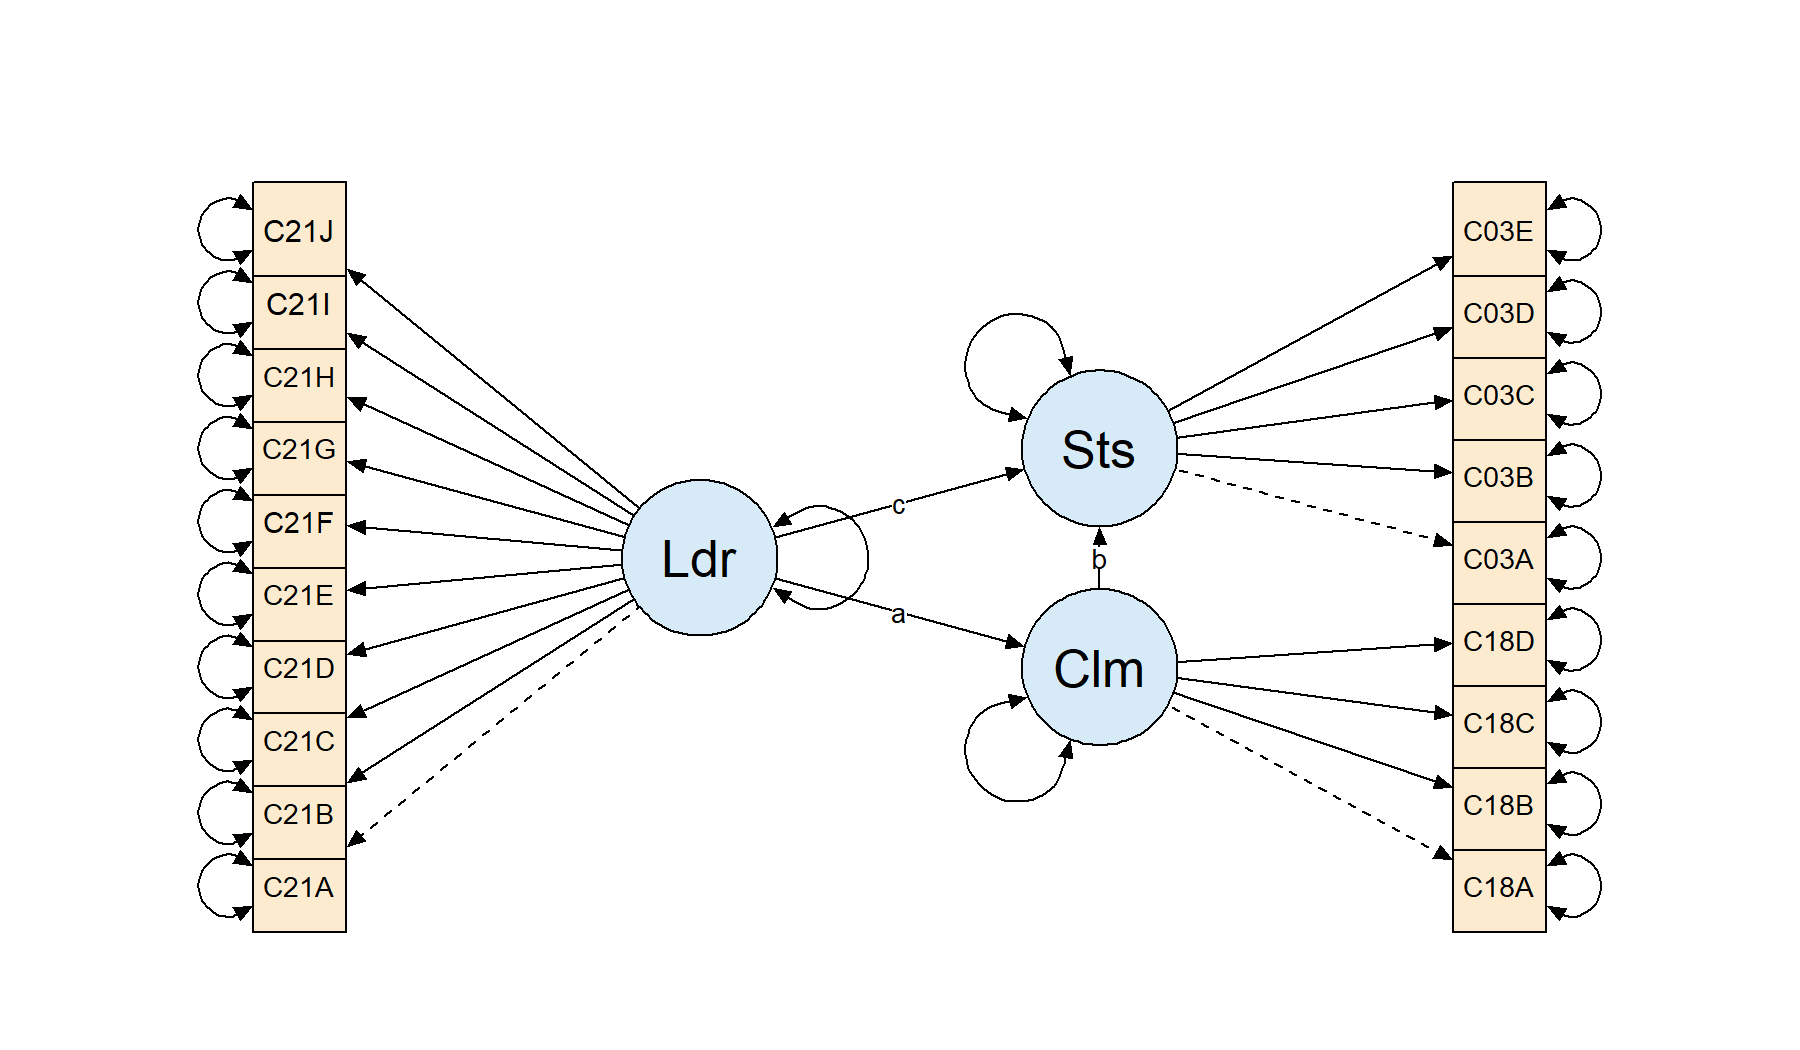
\includegraphics[width=0.62\textwidth]{act6_diagrama_caminos.png}
\caption{Modelo conceptual de mediación parcial entre liderazgo, clima laboral y
satisfacción laboral. Elaborado en la Fase 1 con la sintaxis de \texttt{lavaan}.}
\label{fig:conceptual}
\end{figure}

\begin{description}
\item[H1.] El liderazgo directivo se asocia positivamente con el clima laboral
($\gamma_{11} > 0$). Los directivos que motivan, reconocen y tratan con equidad generan
redes de trabajo basadas en el respeto y la confianza \citep{schneider2013}.
\item[H2.] El clima laboral se asocia positivamente con la satisfacción laboral
($\beta_{21} > 0$). Un entorno de compañeros competentes y relaciones respetuosas reduce el
desgaste afectivo e incrementa el bienestar \citep{carr2003,parker2003}.
\item[H3.] El liderazgo directivo se asocia positivamente con la satisfacción laboral por
una vía directa ($\gamma_{21} > 0$). El apoyo y el ejemplo del superior fortalecen el
sentido de pertenencia y el orgullo institucional \citep{judge2004}.
\item[H4.] El clima laboral media parcialmente la relación entre liderazgo y satisfacción
($\gamma_{11}\beta_{21} > 0$), de modo que el efecto indirecto es positivo y distinto de
cero \citep{walumbwa2008}.
\end{description}

La distinción entre mediación total y parcial es sustantiva: si H3 se sostiene, el
liderazgo conserva un efecto propio sobre la satisfacción y el clima actúa como mecanismo
complementario; si H3 no se sostiene, el clima sería el canal exclusivo. El modelo se
especifica, por tanto, como mediación parcial y se contrasta frente a una versión sin la
ruta directa (sección~\ref{sec:resultados}).

% =====================================================================
\section{Datos}\label{sec:datos}
% =====================================================================

\subsection{Fuente, población e instrumento}

La fuente primaria es la microbase anonimizada de la EDI 2025, descargada del repositorio
de microdatos del DANE \citep{dane2025}. La unidad de observación es el servidor público
individual vinculado a entidades del Estado colombiano en el ámbito nacional. La base cruda
contiene 26.742 filas y 243 columnas; la muestra analítica conserva las 26.742
observaciones. La Tabla~\ref{tab:ficha} resume la ficha técnica.

\begin{table}[htbp]
\centering
\caption{Ficha técnica de la operación estadística EDI 2025 (DANE).}
\label{tab:ficha}
\small
\begin{tabularx}{\textwidth}{@{}lX@{}}
\toprule
Campo & Especificación \\
\midrule
Entidad responsable & Departamento Administrativo Nacional de Estadística (DANE) \\
Operación estadística & Encuesta sobre Ambiente y Desempeño Institucional (EDI), sector público \\
Año de referencia & 2025 \\
Cobertura & Nacional: ramas ejecutiva, legislativa, judicial y organismos de control \\
Diseño muestral & Probabilístico, estratificado por sector institucional y grupo funcional \\
Base cruda & 26.742 filas $\times$ 243 columnas \\
Muestra analítica & 26.742 servidores públicos \\
Clúster de análisis & 201 entidades (variable \texttt{COD\_ENT}) \\
Variables de diseño & \texttt{CODSECTOR}, \texttt{CODGRUPO}, \texttt{FEXPFINAL} \\
Identificador institucional & \texttt{CUIN} (1.711 faltantes en la fuente; no es llave primaria) \\
Sociodemográfica & \texttt{B04}: sexo (1 = hombre, 2 = mujer) \\
Instrumento & 19 indicadores ordinales Likert de 1 a 5 \\
\bottomrule
\end{tabularx}
\end{table}

Los 19 indicadores se agrupan en tres módulos: C21 (liderazgo, 10 ítems), C18 (clima, 4
ítems) y C03 (satisfacción, 5 ítems). Todos emplean una escala Likert de cinco categorías
(1 = nunca o totalmente en desacuerdo; 5 = siempre o totalmente de acuerdo). El Apéndice~\ref{ap:dict}
presenta el diccionario completo.

\subsection{Procesamiento y flujo de registros}

El procesamiento se implementó en R con rutas relativas, semilla fija y registro de
sesión. La Tabla~\ref{tab:flujo} documenta el flujo: no se eliminó ningún registro. La
variable \texttt{CUIN} identifica la entidad y no al servidor, de modo que sus repeticiones
no constituyen duplicados; se conservaron los 1.711 casos con \texttt{CUIN} vacío y se
asignaron al clúster según \texttt{COD\_ENT}. Los códigos especiales de la encuesta (9, 99,
98, 88 y $-1$) se recodificaron como valores perdidos. El ítem C03F se excluyó del
constructo por medir sobrecarga (sentido inverso) y no satisfacción; permanece en la base,
pero no entra en el modelo.

\begin{table}[htbp]
\centering
\caption{Flujo de registros en la construcción de la base analítica.}
\label{tab:flujo}
\small
\begin{tabular}{@{}llrr@{}}
\toprule
Paso & Criterio & $n$ & Eliminados \\
\midrule
0 & Base cruda original & 26.742 & --- \\
1 & Selección de variables (243 $\rightarrow$ 26 columnas) & 26.742 & 0 \\
2 & Diagnóstico de \texttt{CUIN} (identifica entidad) & 26.742 & 0 \\
3 & Filtro de sexo reportado (\texttt{B04}) & 26.742 & 0 \\
4 & Filtro de al menos un ítem respondido & 26.742 & 0 \\
\bottomrule
\end{tabular}
\end{table}

\subsection{Calidad de los datos: faltantes, atípicos y normalidad}

\textbf{Faltantes.} El porcentaje de valores perdidos por indicador es bajo: entre 0,19\,\%
(C03E) y 4,49\,\% (C21I). A nivel de observación, 23.497 servidores (87,87\,\%) completaron
los 20 ítems y 21 casos (0,08\,\%) presentaron faltantes en el 100\,\% de los indicadores.
La prueba de Little rechazó el mecanismo completamente aleatorio
($\chi^2$ = 17.677,7; \df{} = 11.007; $p < 0,001$), por lo que se asumió un mecanismo
aleatorio condicional (MAR) o no aleatorio (MNAR) y se adoptó el tratamiento por pares que
acompaña al estimador ordinal, con análisis de sensibilidad en la sección~\ref{sec:resultados}
\citep{enders2022,little1988}.

La Figura~\ref{fig:faltantes} resume el patrón de faltantes por ítem.

\begin{figure}[htbp]
\centering
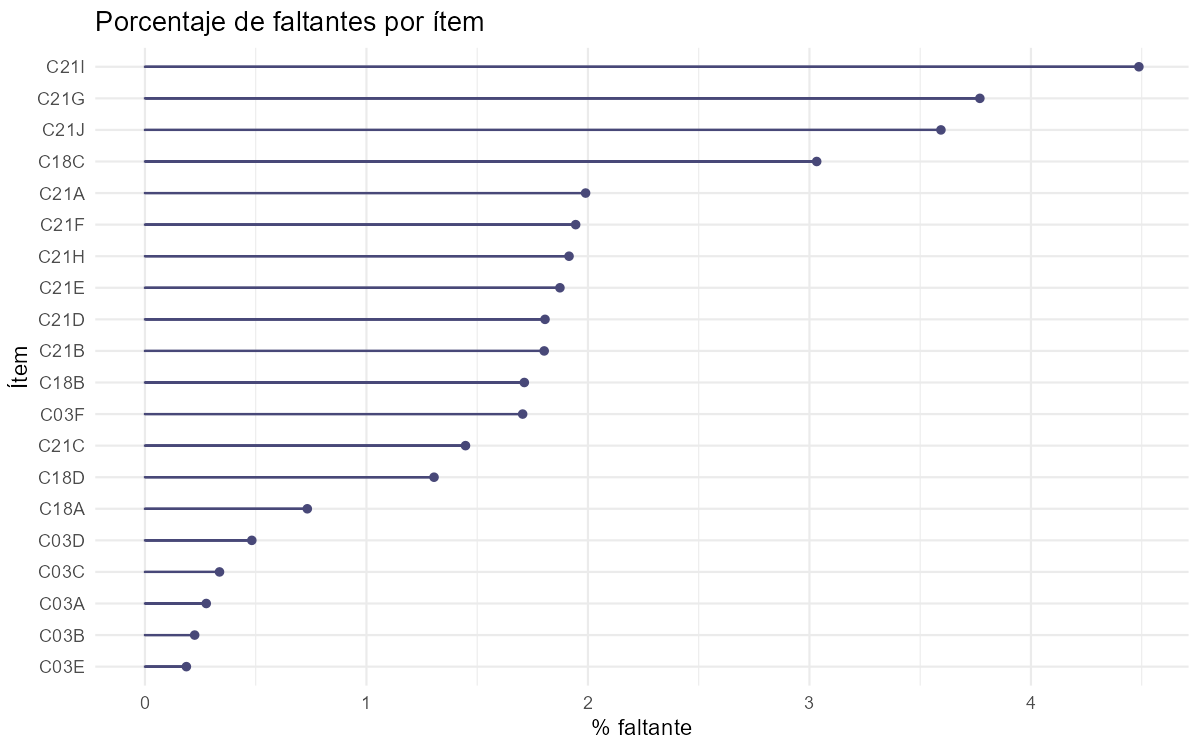
\includegraphics[width=0.55\textwidth]{act3_faltantes_por_item.png}
\caption{Porcentaje de datos faltantes por ítem en la base analítica ($n$ = 26.742).}
\label{fig:faltantes}
\end{figure}

\textbf{Atípicos.} El z robusto basado en la mediana y la desviación absoluta mediana no fue
informativo, porque varios ítems ordinales presentan MAD = 0. Sobre los 23.497 casos
completos y con un umbral $\chi^2_{0,999;\,20}$ = 45,31 se identificaron 2.261
observaciones atípicas multivariadas (9,62\,\%); se interpretaron como patrones extremos
legítimos y se conservaron. Se detectaron 1.011 casos (3,78\,\%) con respuesta idéntica en
todos los ítems (62,3\,\% en la categoría 5 y 32,5\,\% en la categoría 4), que también se
conservaron para preservar la representatividad y se examinan como análisis de sensibilidad.

\textbf{Normalidad multivariada.} La prueba de Mardia sobre 23.760 casos completos rechazó
la normalidad: asimetría $b_{1,p}$ = 47,2086 ($\chi^2$ = 186.946,1; \df{} = 1.330;
$p < 0,001$) y curtosis $b_{2,p}$ = 762,5252 ($z$ = 991,8051; $p < 0,001$), frente a un
valor esperado de 399 bajo normalidad \citep{mardia1970}. Este resultado, junto con la
naturaleza ordinal de los indicadores, determinó el uso de WLSMV.

\subsection{Síntesis psicométrica de la Fase 1}

La Tabla~\ref{tab:descriptivos} resume los estadísticos descriptivos. Los promedios son
altos (entre 3,89 en C21A y 4,62 en C03E) y las desviaciones estándar oscilan entre 0,58 y
1,10. La asimetría es negativa en todos los ítems y la curtosis se mantiene por debajo de 7,
aunque el patrón es claramente no normal. Los efectos techo son severos: 66,2\,\% en C03B y
65,8\,\% en C03E, mientras el efecto piso es marginal (inferior a 4,41\,\%). Esta asimetría
es consistente con deseabilidad social en encuestas de percepción del sector público
(Figura~\\ref{fig:pisotecho}).

\begin{figure}[htbp]
\centering
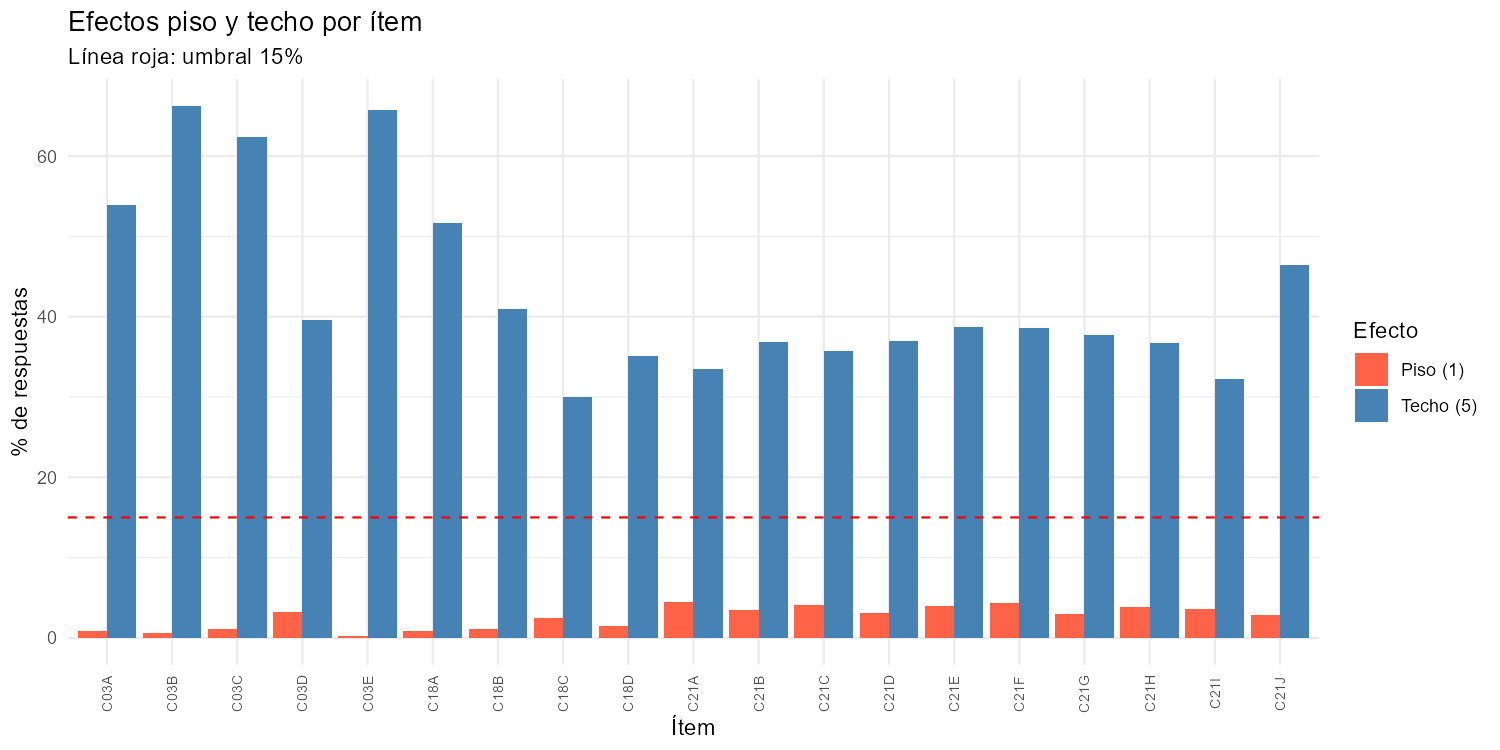
\includegraphics[width=0.58\textwidth]{act4_piso_techo.png}
\caption{Efectos piso (categoría 1) y techo (categoría 5) por ítem. La línea punteada marca el
umbral del 15\,\%.}
\label{fig:pisotecho}
\end{figure}

\begin{table}[htbp]
\centering
\caption{Estadísticos descriptivos de los 19 indicadores ($n$ = 26.742).}
\label{tab:descriptivos}
\small
\begin{tabular}{@{}llrrrrrr@{}}
\toprule
Constructo & Ítem & Media & D.E. & Mediana & Asimetría & Curtosis & \% techo \\
\midrule
Clima & C18A & 4,37 & 0,79 & 5,00 & $-1,54$ & 2,97 & 51,6 \\
      & C18B & 4,18 & 0,87 & 4,00 & $-1,17$ & 1,45 & 41,0 \\
      & C18C & 3,92 & 0,96 & 4,00 & $-0,85$ & 0,55 & 30,0 \\
      & C18D & 4,11 & 0,86 & 4,00 & $-1,09$ & 1,57 & 35,1 \\
Liderazgo & C21A & 3,89 & 1,10 & 4,00 & $-0,98$ & 0,29 & 33,5 \\
      & C21B & 4,02 & 1,02 & 4,00 & $-1,15$ & 0,98 & 36,9 \\
      & C21C & 3,95 & 1,07 & 4,00 & $-1,01$ & 0,52 & 35,7 \\
      & C21D & 4,03 & 0,99 & 4,00 & $-1,13$ & 1,06 & 37,0 \\
      & C21E & 4,03 & 1,04 & 4,00 & $-1,18$ & 1,02 & 38,7 \\
      & C21F & 4,00 & 1,07 & 4,00 & $-1,11$ & 0,73 & 38,5 \\
      & C21G & 4,05 & 0,98 & 4,00 & $-1,13$ & 1,14 & 37,7 \\
      & C21H & 3,99 & 1,04 & 4,00 & $-1,09$ & 0,81 & 36,7 \\
      & C21I & 3,90 & 1,04 & 4,00 & $-0,89$ & 0,41 & 32,2 \\
      & C21J & 4,22 & 0,95 & 4,00 & $-1,48$ & 2,22 & 46,5 \\
Satisfacción & C03A & 4,41 & 0,77 & 5,00 & $-1,61$ & 3,41 & 53,9 \\
      & C03B & 4,58 & 0,68 & 5,00 & $-1,99$ & 5,27 & 66,2 \\
      & C03C & 4,48 & 0,80 & 5,00 & $-1,85$ & 3,84 & 62,3 \\
      & C03D & 4,05 & 1,03 & 4,00 & $-1,18$ & 0,95 & 39,6 \\
      & C03E & 4,62 & 0,58 & 5,00 & $-1,70$ & 4,66 & 65,8 \\
\bottomrule
\end{tabular}
\end{table}

\textbf{Estructura exploratoria.} La matriz de correlaciones policóricas (19 $\times$ 19)
resultó definida positiva (determinante $2{,}305 \times 10^{-9}$; Figura~\ref{fig:poli}). Las
correlaciones medias dentro de cada constructo (0,777 en liderazgo; 0,748 en clima; 0,606 en
satisfacción) superaron las correlaciones medias entre constructos (0,536, 0,435 y 0,412), lo
que aporta evidencia preliminar de convergencia y discriminación. La adecuación muestral fue
excelente (KMO = 0,963) y la prueba de esfericidad de Bartlett fue significativa
($\chi^2$ = 531.682,7; \df{} = 171; $p < 0,001$). El análisis paralelo de Horn sugirió tres
factores \citep{horn1965}. El análisis factorial exploratorio con extracción de mínimos
residuos y rotación oblimin reprodujo la estructura hipotetizada, sin cargas cruzadas
superiores a 0,30 (Figura~\ref{fig:afe}), y explicó el 73,5\,\% de la varianza total.

La consistencia interna fue alta: $\alpha$ de Cronbach de 0,956 (liderazgo), 0,876 (clima) y
0,795 (satisfacción); $\omega$ de McDonald de 0,958, 0,881 y 0,822, respectivamente
\citep{cronbach1951,mcdonald1999}. Estos resultados justificaron el paso al modelo
confirmatorio.

\begin{figure}[htbp]
\centering
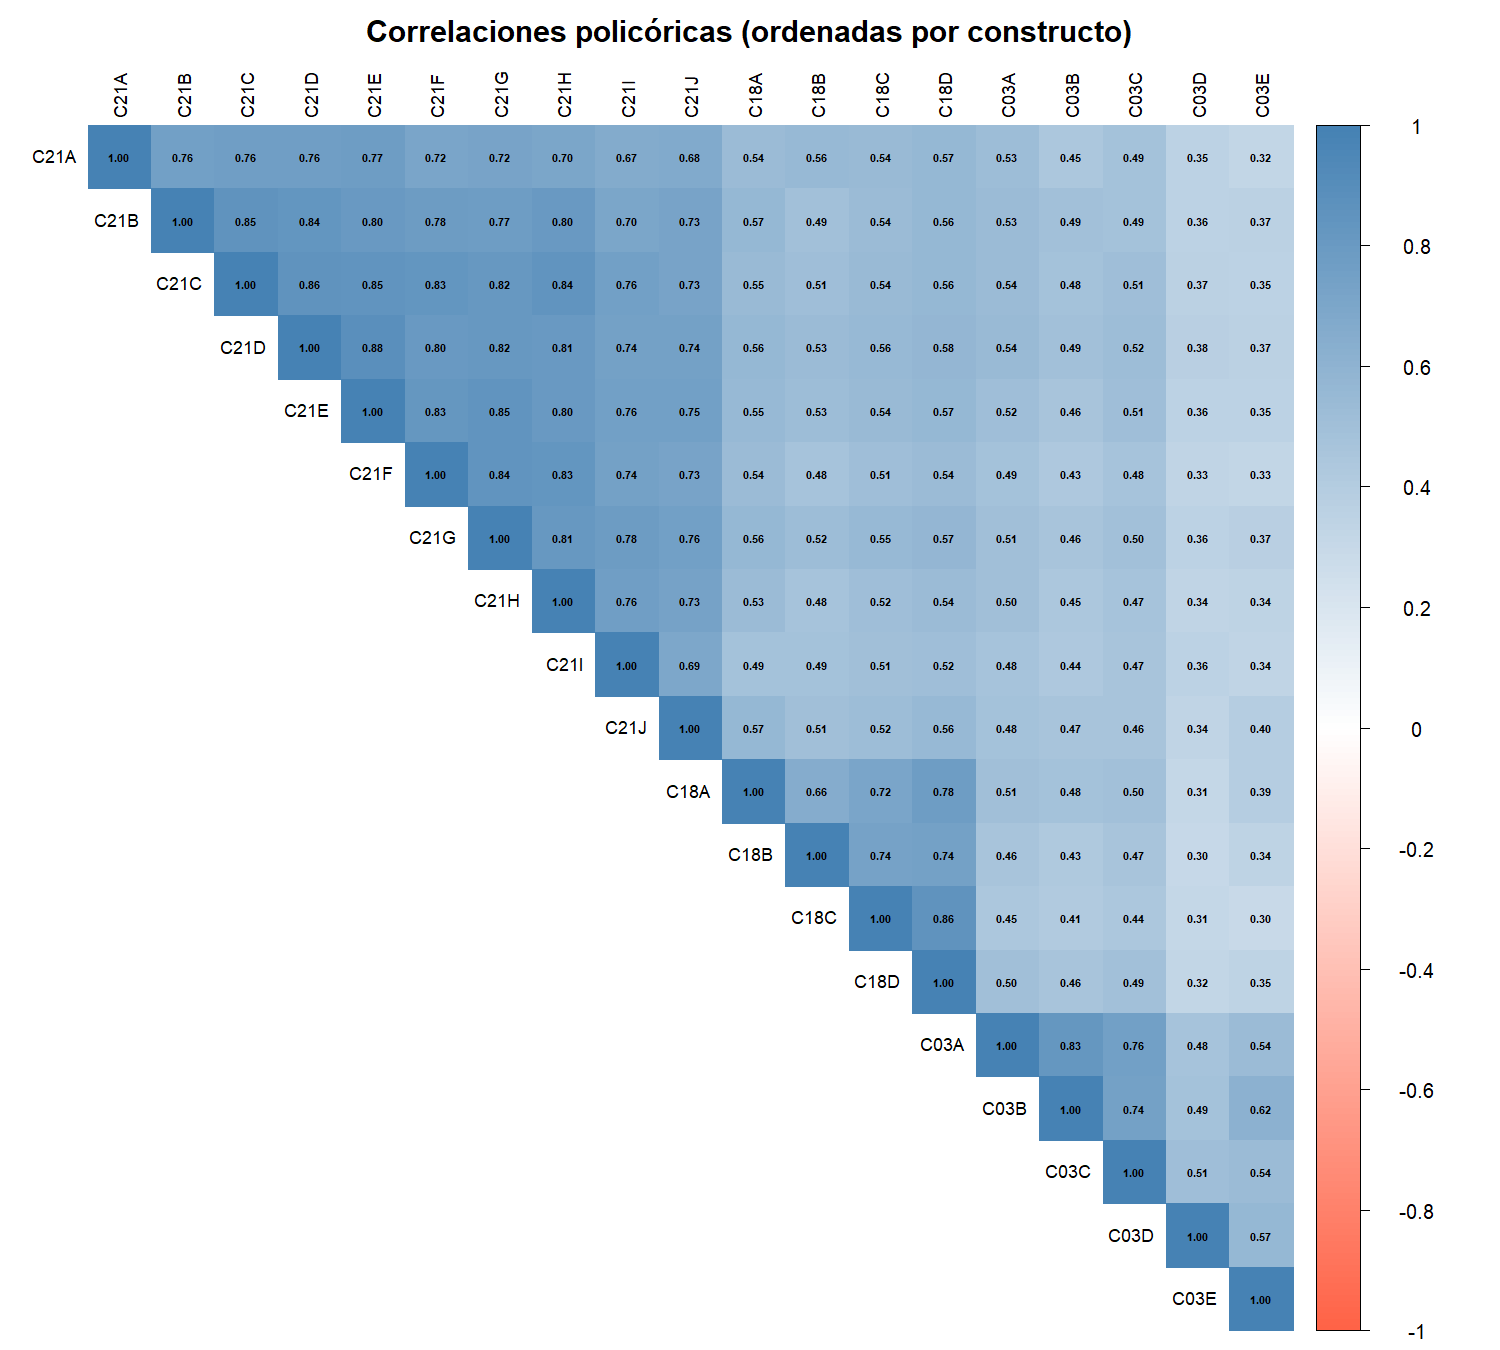
\includegraphics[width=0.55\textwidth]{act5_mapa_calor_poli.png}
\caption{Matriz de correlaciones policóricas ordenada por constructo.}
\label{fig:poli}
\end{figure}

\begin{figure}[htbp]
\centering
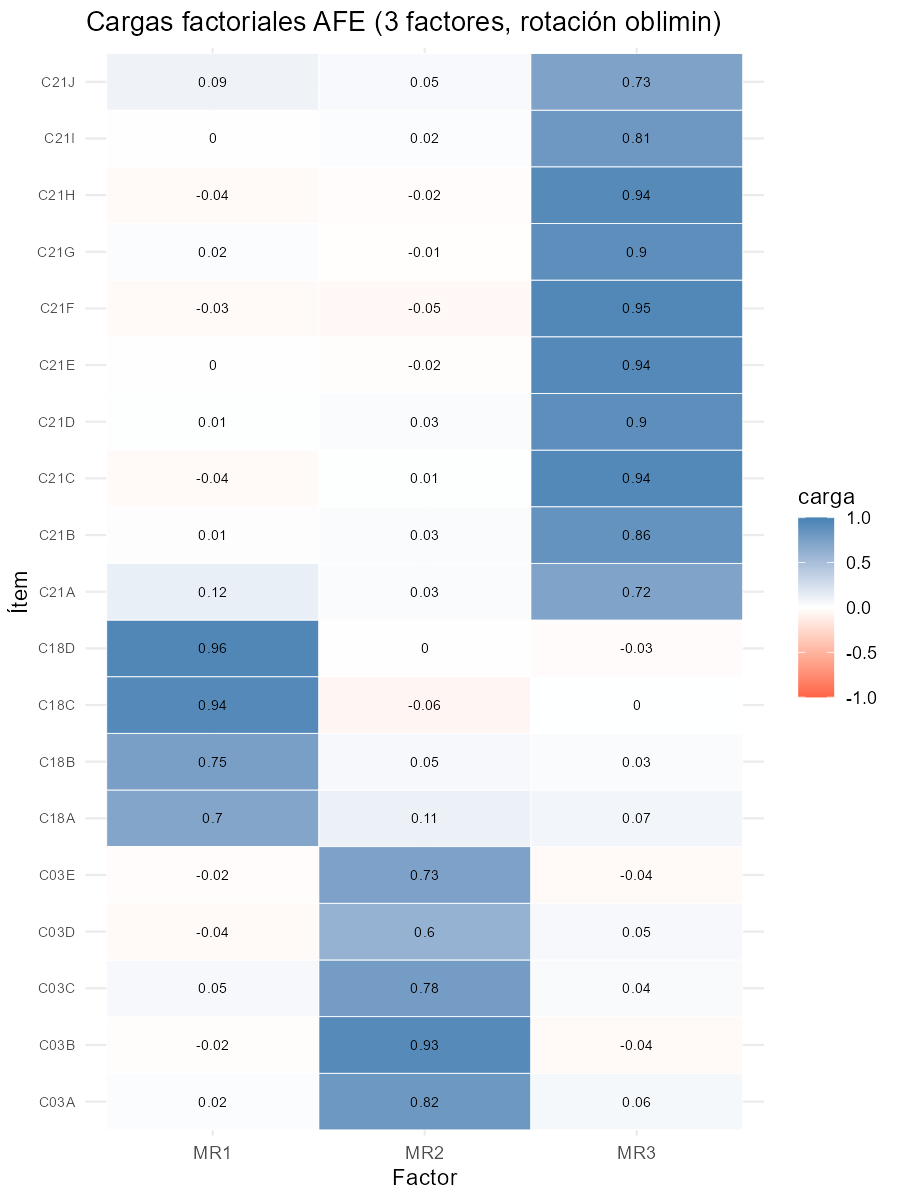
\includegraphics[width=0.48\textwidth]{act5_cargas_afe.png}
\caption{Cargas factoriales del análisis exploratorio de tres factores con rotación
oblimin.}
\label{fig:afe}
\end{figure}

% =====================================================================
\section{Métodos}\label{sec:metodos}
% =====================================================================

\subsection{Especificación del modelo}

Sea $\boldsymbol{\eta} = (\eta_1, \eta_2)'$ el vector de variables latentes endógenas
(clima laboral y satisfacción laboral) y $\xi$ la variable latente exógena (liderazgo). El
modelo de medición se escribe, en notación LISREL \citep{bollen1989}:
\begin{align}
\mathbf{x} &= \boldsymbol{\Lambda}_x \xi + \boldsymbol{\delta}, \label{eq:x}\\
\mathbf{y} &= \boldsymbol{\Lambda}_y \boldsymbol{\eta} + \boldsymbol{\varepsilon}, \label{eq:y}
\end{align}
donde $\mathbf{x}$ contiene los diez indicadores de liderazgo, $\mathbf{y}$ los nueve
indicadores de clima y satisfacción, y $\boldsymbol{\delta}$ y $\boldsymbol{\varepsilon}$
son los errores de medición. El modelo estructural es:
\begin{equation}
\boldsymbol{\eta} = \mathbf{B}\boldsymbol{\eta} + \boldsymbol{\Gamma}\xi + \boldsymbol{\zeta},
\label{eq:est}
\end{equation}
con
\begin{equation}
\mathbf{B} = \begin{pmatrix} 0 & 0 \\ \beta_{21} & 0 \end{pmatrix}, \qquad
\boldsymbol{\Gamma} = \begin{pmatrix} \gamma_{11} \\ \gamma_{21} \end{pmatrix}.
\label{eq:matrices}
\end{equation}
La ecuación~\eqref{eq:est} implica $\eta_1 = \gamma_{11}\xi + \zeta_1$ (clima) y
$\eta_2 = \beta_{21}\eta_1 + \gamma_{21}\xi + \zeta_2$ (satisfacción). El efecto indirecto
es $\gamma_{11}\beta_{21}$ y el total $\gamma_{21} + \gamma_{11}\beta_{21}$.

\subsection{Identificación}

Con $k = 19$ indicadores existen $k(k+1)/2 = 190$ momentos muestrales. El modelo de medición
saturado (tres factores correlacionados) tiene 41 parámetros libres, de modo que
$\df = 190 - 41 = 149$: está sobreidentificado. La escala de cada factor se fijó con el
indicador marcador (C21A = C18A = C03A = 1), coherente con la notación LISREL de la Fase 1.
Cada factor tiene al menos tres indicadores y la matriz $\mathbf{B}$ es triangular inferior,
lo que satisface la regla de los tres indicadores y la condición recursiva.

Una precisión importante: el modelo estructural de mediación parcial reemplaza las tres
covarianzas entre factores por tres coeficientes ($\gamma_{11}$, $\beta_{21}$,
$\gamma_{21}$), de modo que conserva 41 parámetros libres y 149 \df. El bloque estructural
es, por tanto, saturado respecto del modelo de medición.

\subsection{Estimador y tratamiento de los faltantes}

Los indicadores son ordinales de cinco categorías y la prueba de Mardia rechazó la
normalidad multivariada. En consecuencia, el modelo se estimó con WLSMV, que trabaja sobre
la matriz de correlaciones policóricas y los umbrales, y produce errores estándar e índices
de ajuste corregidos \citep{li2016,xia2019}. Los faltantes se trataron por eliminación por
pares, que es el comportamiento por defecto de \texttt{lavaan} con WLSMV; el estimador no
admite información completa (FIML) con datos ordinales \citep{enders2022}.

\subsection{Diseño muestral}

La EDI es una encuesta compleja con estratos por sector y grupo funcional, factor de
expansión y conglomerados por entidad. Para incorporar la conglomeración se declaró
\texttt{cluster = .cluster\_entidad} (201 entidades), lo que produce errores estándar
robustos a la dependencia intra-entidad \citep{oberski2014}. El factor de expansión
(\texttt{FEXPFINAL}) no se combinó con el clúster en el modelo principal, porque
\texttt{lavaan} no admite ambos argumentos simultáneamente con WLSMV; su efecto se evaluó en
un análisis de sensibilidad con un modelo equivalente ponderado por expansión
(sección~\ref{sec:sens}).

\subsection{Índices y criterios de ajuste}

Se reportan \chisq{} escalada, grados de libertad, CFI, TLI, RMSEA con intervalo de confianza
del 90\,\% y SRMR. Los criterios de referencia son CFI y TLI $\geq$ 0,95, RMSEA $\leq$ 0,06
y SRMR $\leq$ 0,08 \citep{hu1999}, sin tratarlos como reglas de oro \citep{marsh2004}. En
todos los modelos con clúster se reportan las versiones escaladas (\textit{scaled}) como
criterio principal, apropiadas para WLSMV \citep{xia2019}, y las robustas como referencia.
La discrepancia entre ambas se discute explícitamente en la sección~\ref{sec:discusion}.

\subsection{Fiabilidad y validez}

Para cada constructo se calculó la fiabilidad compuesta
$\mathrm{CR} = (\sum_j \lambda_j)^2 / [(\sum_j \lambda_j)^2 + \sum_j \theta_j]$ y la varianza
media extraída $\mathrm{AVE} = k^{-1}\sum_j \lambda_j^2$ \citep{fornell1981}. Los criterios de
validez convergente fueron cargas estandarizadas $\geq$ 0,50, CR $\geq$ 0,70 y AVE $\geq$
0,50. La validez discriminante se evaluó con el criterio de Fornell-Larcker —la raíz cuadrada
del AVE debe superar las correlaciones entre constructos— y con la razón
heterorrasgo-monorrasgo (HTMT), que debe ser inferior a 0,85 \citep{henseler2015}.

\subsection{Procedimiento de mediación}

El efecto indirecto se define con el operador \texttt{:=} de \texttt{lavaan} y sus intervalos
de confianza se obtuvieron por dos vías. La primera es la simulación de Monte Carlo
(20.000 réplicas) a partir de la media y la matriz de covarianzas de los estimadores, que
respeta el estimador WLSMV y el clúster \citep{mackinnon2004,preacher2012}. La segunda es un
bootstrap no paramétrico por conglomerados con 2.000 remuestras, que remuestrea entidades
completas y reestima el modelo con MLR, dado que \texttt{lavaan} no implementa bootstrap con
WLSMV para datos ordinales \citep{preacher2008,hayes2022}. Los resultados de esta segunda
vía se reportan como análisis de sensibilidad y se comparan en escala estandarizada.

\subsection{Invarianza}

La invarianza de medición se evaluó con la secuencia de \citet{wu2016} para indicadores
ordinales: configural, umbrales, métrica y escalar. Cada nivel se comparó con el anterior
mediante la diferencia escalada de \chisq{} y los cambios en los índices aproximados; la
invarianza se sostiene si $\Delta$CFI $\geq -0,010$, $\Delta$RMSEA $\leq 0,015$ y
$\Delta$SRMR $\leq 0,030$ en el nivel métrico y $\leq 0,010$ en el escalar
\citep{cheung2002,chen2007,meredith1993,vandenberg2000,putnick2016}. La invarianza
estructural se contrastó igualando los coeficientes entre grupos y aplicando la prueba de
Wald \citep{satorra2001,byrne1989}.

\subsection{Software}

Todos los análisis se ejecutaron en R 4.5.2 \citep{rcore2025} con \texttt{lavaan} 0.7-2
\citep{rosseel2012}, \texttt{semTools} 0.5-9 \citep{jorgensen2022} y \texttt{semPlot}
\citep{epskamp2015}. El pipeline completo, sus decisiones y las correcciones aplicadas se
documentan en \texttt{CORRECCIONES.md}; los scripts están numerados por etapa y se ejecutan
con \texttt{00\_run\_all.R}. La sintaxis completa del modelo aparece en el Apéndice~\ref{ap:sintaxis}.

% =====================================================================
\section{Resultados}\label{sec:resultados}
% =====================================================================

\subsection{Modelo de medición: análisis factorial confirmatorio}

El AFC con tres factores correlacionados convergió en 66 iteraciones, sin varianzas de error
negativas, sin correlaciones entre factores superiores a la unidad y sin cargas
estandarizadas mayores o iguales a uno; el chequeo posterior de \texttt{lavaan} no reportó
soluciones impropias. El ajuste del modelo base fue aceptable, con una mejora sustancial tras
la reespecificación descrita a continuación (Tabla~\ref{tab:ajuste}).

\begin{table}[htbp]
\centering
\caption{Índices de ajuste de los modelos estimados. Se reportan las versiones escaladas
(criterio principal) y robustas (referencia).}
\label{tab:ajuste}
\small
\begin{tabular}{@{}lrrrrrrrr@{}}
\toprule
Modelo & \chisq & \df & CFI & TLI & RMSEA [IC90] & SRMR & CFI$_{rob}$ & RMSEA$_{rob}$ \\
\midrule
AFC base & 9.755,18 & 149 & 0,987 & 0,985 & 0,052 [0,051; 0,053] & 0,028 & 0,958 & 0,075 \\
AFC final & 8.856,34 & 148 & 0,988 & 0,986 & 0,050 [0,049; 0,051] & 0,025 & 0,964 & 0,070 \\
M1 estructural & 8.856,34 & 148 & 0,988 & 0,986 & 0,050 [0,049; 0,051] & 0,025 & 0,964 & 0,070 \\
\bottomrule
\end{tabular}
\end{table}

\textbf{Ajuste local y reespecificación.} El examen de los residuos de correlación mostró que
solo uno de los 171 pares de ítems superó el umbral $|r| > 0,10$: C03D--C03E
($r$ = 0,148). Los índices de modificación coincidieron en señalar ese par como el de mayor
valor (IM = 820,37; EPC = 0,176), por encima de la covarianza C18C--C18D (IM = 740,73) y de
las cargas cruzadas sugeridas entre factores. Ambos ítems pertenecen al constructo de
satisfacción y comparten una redacción afín —extender la jornada y dar el mejor esfuerzo—,
por lo que se liberó una única covarianza residual entre sus errores, con justificación
teórica y de a un parámetro a la vez \citep{kline2023,maccallum1992}. La reespecificación
redujo la \chisq{} en 898,84 puntos con un grado de libertad y mejoró el CFI de 0,987 a
0,988 y el SRMR de 0,028 a 0,025.

Para reducir el riesgo de capitalizar el azar, la muestra se dividió aleatoriamente
(semilla 2026) en calibración ($n$ = 18.719) y validación ($n$ = 8.023). El modelo
reespecificado se estimó en calibración (CFI = 0,990; TLI = 0,988; RMSEA = 0,050;
SRMR = 0,025) y se confirmó en validación (CFI = 0,991; TLI = 0,990; RMSEA = 0,052;
SRMR = 0,026), con $\Delta$CFI = 0,001 y $\Delta$RMSEA = 0,001. La reespecificación se
sostiene fuera de la muestra de calibración.

La Figura~\ref{fig:afc} presenta el modelo de medición final con las cargas estandarizadas.

\begin{figure}[htbp]
\centering
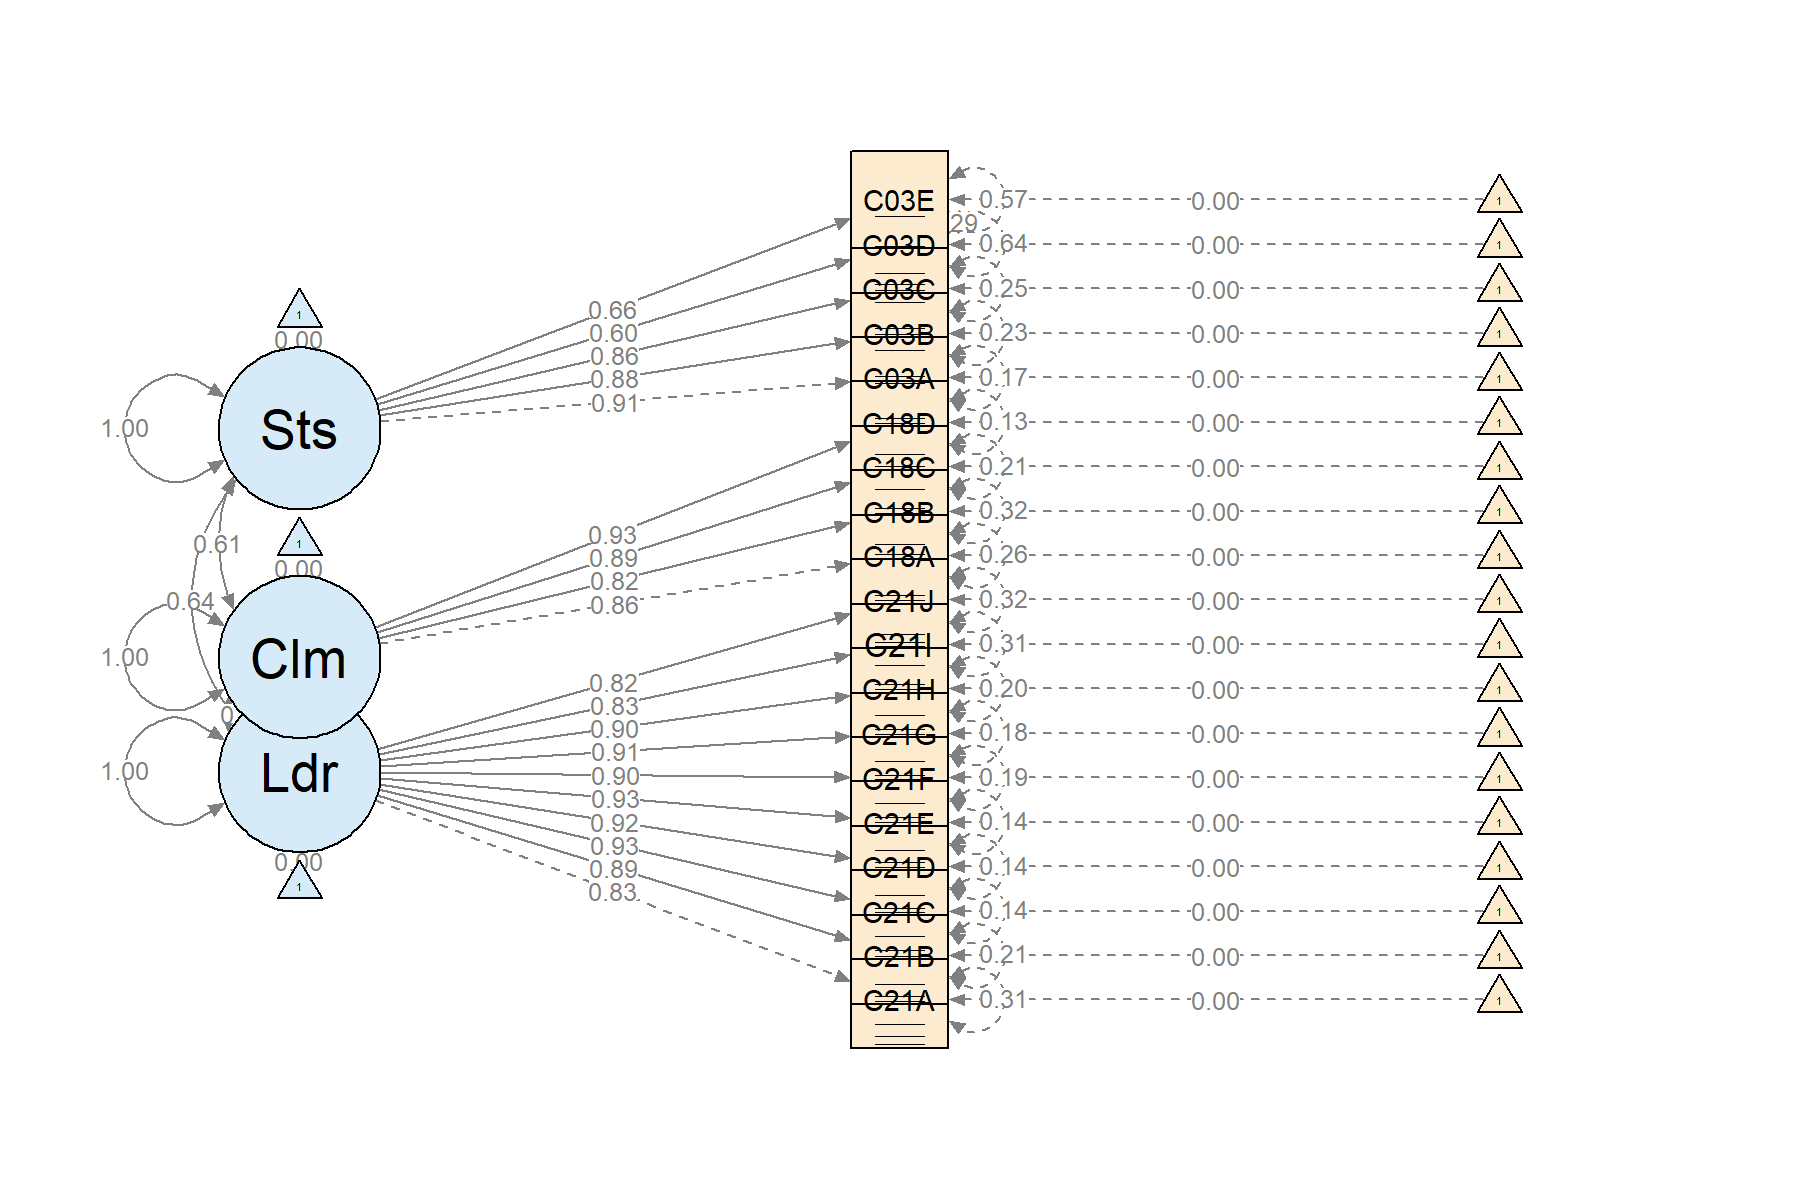
\includegraphics[width=0.68\textwidth]{act9_afc_final.png}
\caption{Modelo de medición final con cargas estandarizadas. La curva entre C03D y C03E
representa la covarianza residual liberada.}
\label{fig:afc}
\end{figure}

\subsection{Cargas, fiabilidad y validez}

Todas las cargas estandarizadas fueron significativas ($p < 0,001$) y superiores a 0,50
(Tabla~\ref{tab:cargas}). Las diez cargas de liderazgo se ubicaron entre 0,824 y 0,927; las
de clima entre 0,823 y 0,931; en satisfacción, C03A, C03B y C03C presentaron valores altos
(0,911, 0,878 y 0,864), mientras C03D (0,623) y C03E (0,680) fueron las más bajas, en
coherencia con la covarianza residual que comparten.

\begin{table}[htbp]
\centering
\caption{Cargas estandarizadas del AFC final ($n$ = 26.742).}
\label{tab:cargas}
\small
\begin{tabular}{@{}llrrr@{}}
\toprule
Constructo & Ítem & $\lambda$ & E.E. & $z$ \\
\midrule
Liderazgo & C21A & 0,829 & 0,003 & 295,19 \\
          & C21B & 0,892 & 0,002 & 543,05 \\
          & C21C & 0,926 & 0,001 & 628,74 \\
          & C21D & 0,925 & 0,001 & 676,23 \\
          & C21E & 0,927 & 0,001 & 711,14 \\
          & C21F & 0,898 & 0,002 & 524,83 \\
          & C21G & 0,907 & 0,002 & 535,67 \\
          & C21H & 0,897 & 0,002 & 488,51 \\
          & C21I & 0,829 & 0,003 & 290,58 \\
          & C21J & 0,824 & 0,003 & 292,10 \\
Clima     & C18A & 0,861 & 0,004 & 225,81 \\
          & C18B & 0,823 & 0,003 & 254,34 \\
          & C18C & 0,889 & 0,003 & 346,68 \\
          & C18D & 0,931 & 0,002 & 515,73 \\
Satisfacción & C03A & 0,911 & 0,003 & 333,13 \\
          & C03B & 0,878 & 0,003 & 267,99 \\
          & C03C & 0,864 & 0,004 & 214,99 \\
          & C03D & 0,623 & 0,007 & 89,56 \\
          & C03E & 0,680 & 0,006 & 111,16 \\
\bottomrule
\end{tabular}
\end{table}

La fiabilidad compuesta fue 0,973 para liderazgo, 0,930 para clima y 0,892 para satisfacción;
la AVE fue 0,785, 0,769 y 0,628, respectivamente (Tabla~\ref{tab:fiabilidad}). Todos los
constructos superan los umbrales de 0,70 y 0,50.

\begin{table}[htbp]
\centering
\caption{Fiabilidad y validez convergente por constructo.}
\label{tab:fiabilidad}
\small
\begin{tabular}{@{}lrrrrrr@{}}
\toprule
Constructo & $k$ & $\alpha$ & $\omega$ & CR & AVE & $\sqrt{\mathrm{AVE}}$ \\
\midrule
Liderazgo & 10 & 0,956 & 0,958 & 0,973 & 0,785 & 0,886 \\
Clima laboral & 4 & 0,876 & 0,881 & 0,930 & 0,769 & 0,877 \\
Satisfacción laboral & 5 & 0,795 & 0,822 & 0,892 & 0,628 & 0,792 \\
\bottomrule
\end{tabular}
\end{table}

La validez discriminante se cumple por ambos criterios (Tabla~\ref{tab:discriminante}): la
raíz cuadrada del AVE de cada constructo supera sus correlaciones con los demás y los tres
valores de HTMT quedan por debajo de 0,85, con un máximo de 0,703 entre liderazgo y clima.

\begin{table}[htbp]
\centering
\caption{Validez discriminante: criterio de Fornell-Larcker (diagonal en $\sqrt{\mathrm{AVE}}$,
correlaciones bajo la diagonal) y HTMT.}
\label{tab:discriminante}
\small
\begin{tabular}{@{}lcccc@{}}
\toprule
 & Liderazgo & Clima & Satisfacción & HTMT \\
\midrule
Liderazgo & \textbf{0,886} & 0,698 & 0,638 & --- \\
Clima & 0,698 & \textbf{0,877} & 0,614 & 0,703 \\
Satisfacción & 0,638 & 0,614 & \textbf{0,792} & 0,633 / 0,611 \\
\bottomrule
\end{tabular}

\vspace{2pt}
\parbox{0.9\textwidth}{\footnotesize \textit{Nota.} HTMT: liderazgo-clima = 0,703;
liderazgo-satisfacción = 0,633; clima-satisfacción = 0,611.}
\end{table}

\subsection{Modelo estructural}

El modelo M1 reprodujo exactamente el ajuste del AFC final (Tabla~\ref{tab:ajuste}): ambos
tienen \chisq{} = 8.856,34 con 148 \df. La prueba de diferencia escalada arrojó
$\Delta\df = 0$ y $\Delta\chi^2 = -0,001$, de modo que la comparación es
\textbf{no informativa}: al ser el bloque estructural saturado, no existe una restricción
estructural contrastable frente al modelo de medición. Este resultado no indica un mal
ajuste ni un rechazo de la teoría; simplemente refleja que M1 es una reparametrización
equivalente del AFC saturado.

La Tabla~\ref{tab:hipotesis} presenta el contraste de las cuatro hipótesis. Los cuatro
coeficientes son positivos y significativos. H1 (liderazgo $\rightarrow$ clima) presenta el
mayor efecto ($\beta$ = 0,725; $\beta_{est}$ = 0,698), seguido de H3 (liderazgo
$\rightarrow$ satisfacción; $\beta$ = 0,447; $\beta_{est}$ = 0,407) y de H2 (clima
$\rightarrow$ satisfacción; $\beta$ = 0,349; $\beta_{est}$ = 0,330). El efecto indirecto
(H4) es 0,253 ($\beta_{est}$ = 0,230). Dado que las hipótesis especifican signo positivo, se
reporta el valor $p$ unilateral; en los cuatro casos es inferior a 0,001.

\begin{table}[htbp]
\centering
\caption{Contraste de hipótesis estructurales (M1). Coeficientes no estandarizados y
estandarizados.}
\label{tab:hipotesis}
\small
\begin{tabular}{@{}llrrrrrrl@{}}
\toprule
H & Relación & $\beta$ & E.E. & $z$ & $p$ & $p_{uni}$ & $\beta_{est}$ & Decisión \\
\midrule
H1 & Liderazgo $\rightarrow$ Clima & 0,725 & 0,007 & 107,74 & $<$0,001 & $<$0,001 & 0,698 & Se apoya \\
H2 & Clima $\rightarrow$ Satisfacción & 0,349 & 0,010 & 34,72 & $<$0,001 & $<$0,001 & 0,330 & Se apoya \\
H3 & Liderazgo $\rightarrow$ Satisfacción & 0,447 & 0,010 & 44,98 & $<$0,001 & $<$0,001 & 0,407 & Se apoya \\
H4 & Indirecto $\gamma_{11}\beta_{21}$ & 0,253 & 0,008 & 32,19 & $<$0,001 & $<$0,001 & 0,230 & Se apoya \\
\bottomrule
\end{tabular}
\end{table}

El modelo explica el 48,7\,\% de la varianza del clima laboral y el 46,2\,\% de la varianza
de la satisfacción laboral. La Figura~\ref{fig:estructural} presenta el diagrama de caminos
con coeficientes estandarizados; todas las relaciones estructurales resultaron
significativas y, por tanto, ninguna se marca como no significativa.

\begin{figure}[htbp]
\centering
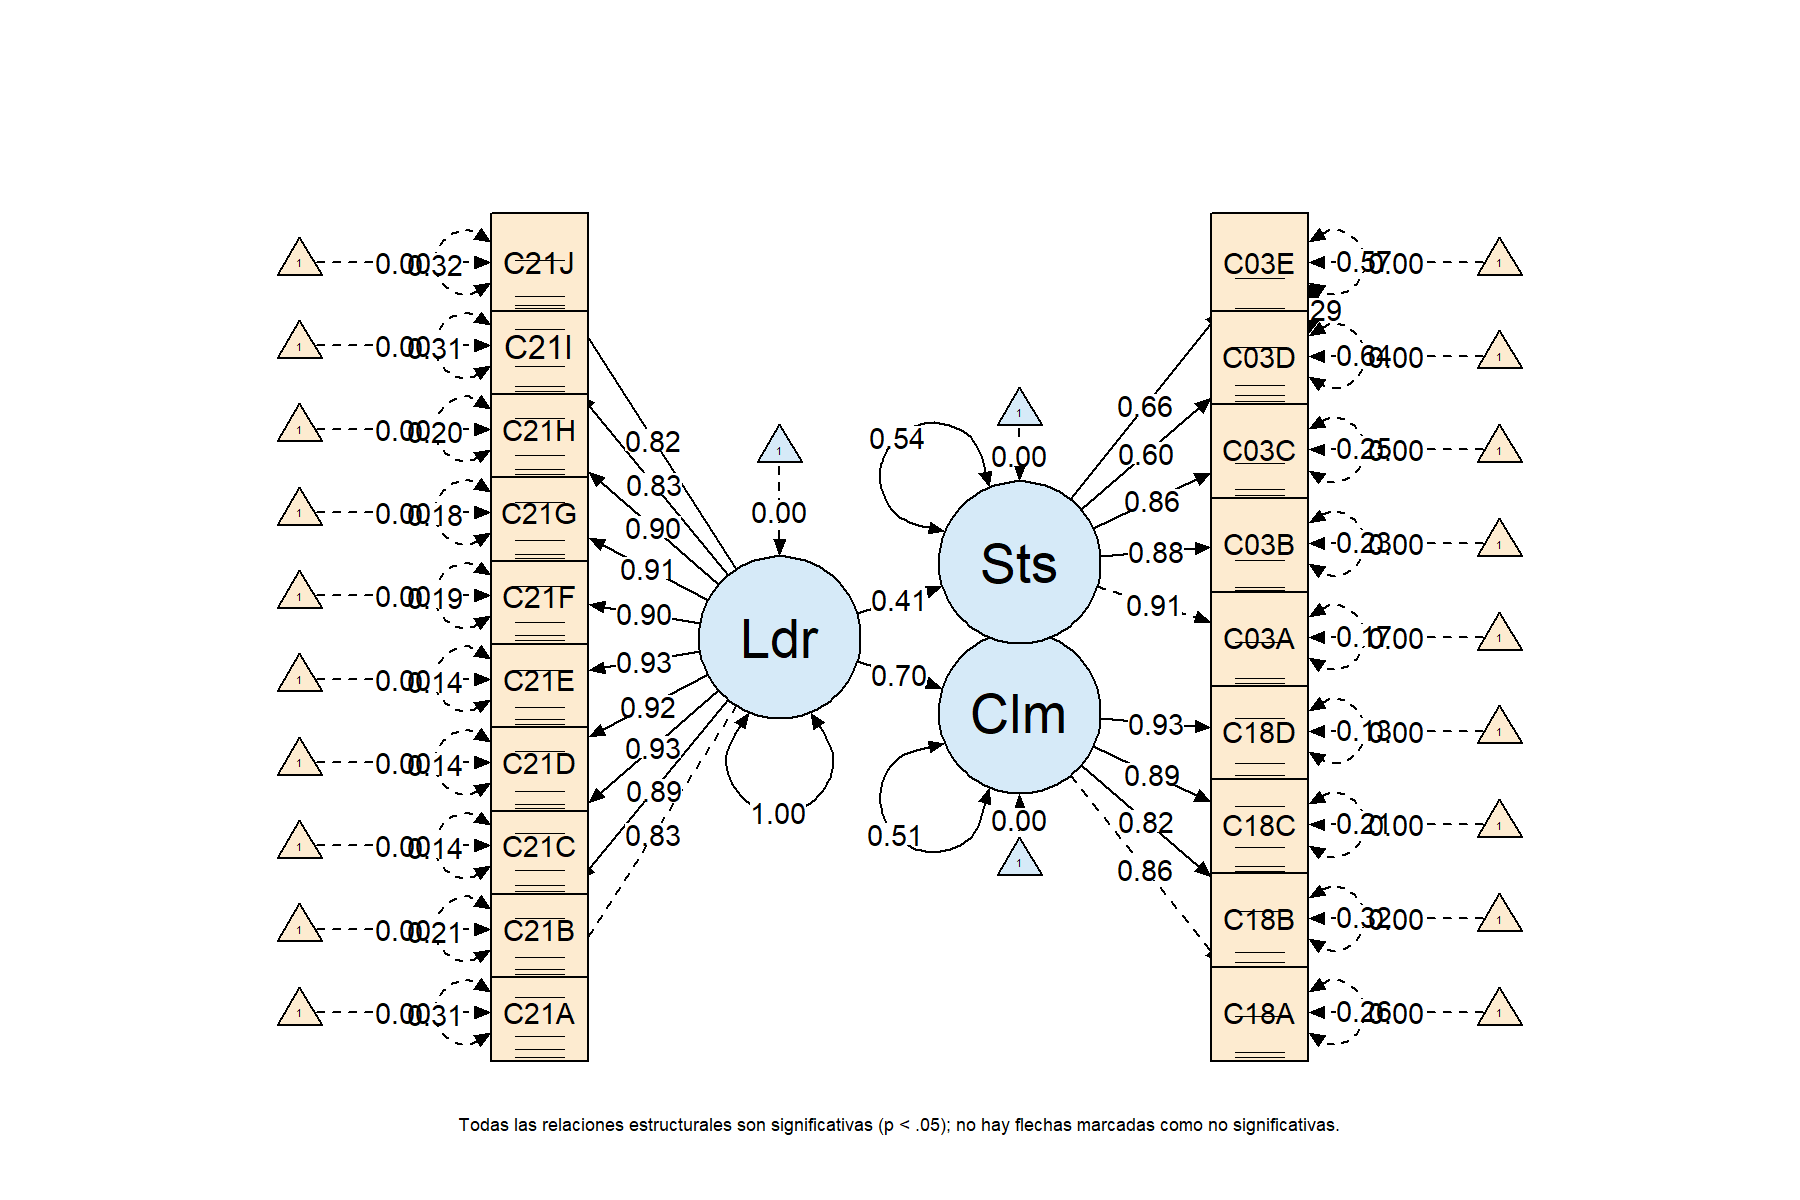
\includegraphics[width=0.72\textwidth]{act12_modelo_estructural.png}
\caption{Modelo estructural M1 con coeficientes estandarizados. Todas las relaciones
estructurales son significativas ($p < 0,05$); la curva entre C03D y C03E corresponde a la
covarianza residual del modelo de medición final.}
\label{fig:estructural}
\end{figure}

\subsection{Efectos directos, indirectos y totales}

La Tabla~\ref{tab:efectos} reporta los efectos con intervalos de confianza por Monte Carlo
(20.000 réplicas, modelo WLSMV) y por bootstrap de conglomerados (2.000 remuestras, modelo
MLR). En ambas vías el efecto indirecto es positivo y su intervalo excluye el cero. El
efecto indirecto representa el 36,1\,\% del efecto total en el modelo WLSMV
(0,253/0,700) y el 34,1\,\% en el modelo MLR (0,147/0,431), lo que confirma una mediación
parcial: la mayor parte del efecto del liderazgo sobre la satisfacción es directa.

\begin{table}[htbp]
\centering
\caption{Efectos directos, indirectos y totales con intervalos de confianza del 95\,\%.
Monte Carlo corresponde al modelo WLSMV; bootstrap, al modelo MLR por conglomerados.}
\label{tab:efectos}
\small
\begin{tabular}{@{}lrrrrrr@{}}
\toprule
 & \multicolumn{2}{c}{Monte Carlo (WLSMV)} & \multicolumn{2}{c}{Bootstrap (MLR)} & \multicolumn{2}{c}{Estandarizado} \\
\cmidrule(lr){2-3}\cmidrule(lr){4-5}\cmidrule(lr){6-7}
Efecto & Est. & IC 95\,\% & Est. & IC 95\,\% & MC & Bootstrap \\
\midrule
Indirecto ($a\cdot b$) & 0,253 & [0,237; 0,268] & 0,147 & [0,135; 0,160] & 0,230 & 0,190 [0,175; 0,207] \\
Directo ($c$) & 0,447 & [0,427; 0,467] & 0,284 & [0,264; 0,303] & 0,407 & --- \\
Total & 0,700 & [0,687; 0,713] & 0,431 & [0,413; 0,449] & 0,638 & --- \\
\bottomrule
\end{tabular}
\end{table}

Las escalas no estandarizadas de ambas vías no son directamente comparables: WLSMV modela
correlaciones policóricas y umbrales, mientras MLR trata los ítems como continuos. Por esa
razón, la comparación sustantiva se hace en unidades estandarizadas: el efecto indirecto es
0,230 con Monte Carlo y 0,190 con bootstrap; las rutas estandarizadas son $a$ = 0,638
[0,623; 0,653] y $b$ = 0,299 [0,276; 0,322] en el bootstrap. Ambas vías coinciden en signo,
en orden de magnitud y en significancia.

\subsection{Modelos alternativos}

La Tabla~\ref{tab:alternativos} compara M1 con tres especificaciones rivales estimadas sobre
el mismo modelo de medición. M2 suprime la ruta directa y deja el clima como mediador total;
M3 invierte la dirección entre liderazgo y clima; M4 propone una cadena
liderazgo $\rightarrow$ satisfacción $\rightarrow$ clima.

\begin{table}[htbp]
\centering
\caption{Comparación de modelos alternativos.}
\label{tab:alternativos}
\small
\begin{tabular}{@{}lrrrrrr@{}}
\toprule
Modelo & \chisq & \df & CFI & TLI & RMSEA & SRMR \\
\midrule
M1: mediación parcial & 8.856,34 & 148 & 0,988 & 0,986 & 0,050 & 0,025 \\
M2: sin mediación (solo efectos directos) & 14.151,71 & 149 & 0,981 & 0,978 & 0,063 & 0,041 \\
M3: dirección opuesta (clima $\rightarrow$ liderazgo) & 14.151,71 & 149 & 0,981 & 0,978 & 0,063 & 0,041 \\
M4: cadena liderazgo $\rightarrow$ satisfacción $\rightarrow$ clima & 25.161,07 & 149 & 0,966 & 0,961 & 0,084 & 0,058 \\
\bottomrule
\end{tabular}
\end{table}

M1 y M2 están anidados: M2 fija en cero la ruta directa. La prueba de diferencia escalada
arrojó $\Delta\chi^2$ = 1.124,77 con un grado de libertad ($p < 0,001$), lo que indica que la
ruta directa aporta información y respalda la mediación parcial frente a la mediación total.
M2 y M3 presentan un ajuste idéntico hasta el segundo decimal y el mismo número de
parámetros: son modelos equivalentes, ajustan igual pero implican direcciones causales
distintas, y solo la teoría puede decidir entre ellos \citep{maccallum1993}. M4, con una
topología distinta, ajusta peor. AIC y BIC no se reportan porque no están definidos para
WLSMV, que es un estimador de mínimos cuadrados y no de máxima verosimilitud; la comparación
entre modelos no anidados se apoya en los índices aproximados y en la teoría.

\subsection{Invarianza de medición por sexo}

La muestra se divide en 12.047 hombres y 14.695 mujeres, ambos grupos muy por encima del
mínimo recomendado. La Tabla~\ref{tab:invsexo} presenta la secuencia de invarianza con
clúster y el criterio de \citet{chen2007}. Los cuatro niveles se sostienen: los cambios en
CFI son positivos o nulos, los de RMSEA negativos y los de SRMR nulos o de 0,001. Las
pruebas de diferencia escalada de \chisq{} resultan significativas en los tres pasos, un
resultado esperable con más de 26.000 observaciones; por esa razón la decisión se apoya en
los cambios de los índices aproximados, tal como recomiendan \citet{cheung2002} y
\citet{chen2007}, y no en el contraste de \chisq{}.

\begin{table}[htbp]
\centering
\caption{Invarianza de medición por sexo (secuencia de Wu y Estabrook, 2016).}
\label{tab:invsexo}
\footnotesize
\setlength{\tabcolsep}{4pt}
\begin{tabular}{@{}lrrrrrrrrrr@{}}
\toprule
Nivel & \chisq & \df & CFI & TLI & RMSEA & SRMR & $\Delta\chi^2$ (\df) & $\Delta$CFI & $\Delta$RMSEA & $\Delta$SRMR \\
\midrule
Configural & 10.272,47 & 298 & 0,989 & 0,987 & 0,053 & 0,028 & --- & --- & --- & --- \\
Umbrales & 6.960,52 & 355 & 0,993 & 0,993 & 0,040 & 0,028 & 146,06 (57) & 0,004 & $-0,013$ & 0,000 \\
Métrico (cargas) & 5.764,06 & 371 & 0,994 & 0,995 & 0,035 & 0,029 & 126,76 (16) & 0,001 & $-0,005$ & 0,001 \\
Escalar (interceptos) & 5.669,89 & 387 & 0,994 & 0,995 & 0,034 & 0,029 & 113,77 (16) & 0,000 & $-0,001$ & 0,000 \\
\bottomrule
\end{tabular}

\vspace{2pt}
\parbox{0.95\textwidth}{\footnotesize \textit{Nota.} Todas las diferencias de $\chi^2$
tienen $p < 0,001$. Umbral de $\Delta$SRMR: 0,030 en el nivel métrico y 0,010 en el escalar
\citep{chen2007}.}
\end{table}

En el nivel escalar, $\Delta$SRMR = 0,000 frente al umbral de 0,010, y los tres criterios se
cumplen simultáneamente en todos los niveles. Puede concluirse que la medición es
equivalente entre hombres y mujeres y que las comparaciones de medias son interpretables.

\subsection{Invarianza estructural por sexo}

Una vez establecida la invarianza escalar, se contrastó la igualdad de los coeficientes
estructurales. El modelo con coeficientes libres y el modelo con coeficientes igualados se
compararon mediante la prueba de Wald: la ruta liderazgo $\rightarrow$ clima difiere entre
sexos ($\chi^2$ = 11,671; \df{} = 1; $p$ = 0,0006), mientras las rutas clima
$\rightarrow$ satisfacción ($\chi^2$ = 3,142; $p$ = 0,076) y liderazgo $\rightarrow$
satisfacción ($\chi^2$ = 2,288; $p$ = 0,130) no muestran diferencias significativas. En
términos sustantivos, la relación entre liderazgo y clima sería ligeramente más intensa en
uno de los grupos, mientras el resto de la estructura permanece estable.

Las medias observadas de los constructos difieren de forma estadísticamente significativa,
aunque con tamaños de efecto pequeños: liderazgo 4,054 en hombres frente a 3,945 en mujeres
($d$ = $-0,123$), clima 4,220 frente a 4,078 ($d$ = $-0,191$) y satisfacción 4,450 frente a
4,413 ($d$ = $-0,064$). Con invarianza escalar, estas diferencias son comparables, pero su
magnitud práctica es limitada.

\subsection{Invarianza por sector}

El análisis por sector incluyó seis sectores con al menos 200 casos, cinco categorías
presentes en todos los ítems y al menos diez entidades por grupo, lo que reunió 11.065 casos.
La secuencia volvió a sostenerse en los cuatro niveles (Tabla~\ref{tab:invsector}), con
$\Delta$CFI entre 0,000 y 0,001 y $\Delta$RMSEA negativos.

\begin{table}[htbp]
\centering
\caption{Invarianza de medición por sector institucional (seis sectores, $n$ = 11.065).}
\label{tab:invsector}
\footnotesize
\setlength{\tabcolsep}{4pt}
\begin{tabular}{@{}lrrrrrrrrrr@{}}
\toprule
Nivel & \chisq & \df & CFI & TLI & RMSEA & SRMR & $\Delta\chi^2$ (\df) & $\Delta$CFI & $\Delta$RMSEA & $\Delta$SRMR \\
\midrule
Configural & 3.391,76 & 894 & 0,993 & 0,992 & 0,039 & 0,031 & --- & --- & --- & --- \\
Umbrales & 3.282,23 & 1.084 & 0,994 & 0,994 & 0,033 & 0,031 & 224,40 (190) & 0,001 & $-0,006$ & 0,000 \\
Métrico (cargas) & 3.075,92 & 1.164 & 0,994 & 0,995 & 0,030 & 0,031 & 108,20 (80) & 0,000 & $-0,003$ & 0,000 \\
Escalar (interceptos) & 2.879,13 & 1.244 & 0,995 & 0,996 & 0,027 & 0,031 & 171,10 (80) & 0,001 & $-0,003$ & 0,000 \\
\bottomrule
\end{tabular}

\vspace{2pt}
\parbox{0.95\textwidth}{\footnotesize \textit{Nota.} Las diferencias de $\chi^2$ tienen
$p$ = 0,044 (umbrales), 0,020 (métrico) y $p < 0,001$ (escalar).}
\end{table}

La prueba de Wald sobre los coeficientes estructurales igualados mostró diferencias entre
sectores en la ruta liderazgo $\rightarrow$ clima ($\chi^2$ = 15,077; \df{} = 5;
$p$ = 0,010; $p$ de Bonferroni = 0,030) y en la ruta clima $\rightarrow$ satisfacción
($\chi^2$ = 14,578; \df{} = 5; $p$ = 0,012; Bonferroni = 0,037), pero no en la ruta directa
liderazgo $\rightarrow$ satisfacción ($\chi^2$ = 6,208; \df{} = 5; $p$ = 0,287). Las medias
por sector oscilaron entre 3,964 y 4,172 en liderazgo, entre 4,086 y 4,326 en clima y entre
4,420 y 4,550 en satisfacción: las diferencias existen, pero son de pequeña magnitud.

\subsection{Análisis multinivel y correlaciones entre entidades}

El CFA multinivel (MLR, dos niveles) permitió descomponer la varianza en componentes dentro y
entre entidades. Los ICC fueron 0,0575 (liderazgo), 0,0500 (clima) y 0,0587 (satisfacción):
alrededor del 5\,\% al 6\,\% de la varianza se atribuye a diferencias entre entidades, lo que
justifica el uso de errores robustos a la conglomeración (Tabla~\ref{tab:multinivel}). El ICC
calculado de forma independiente con modelos nulos de efectos aleatorios sobre los puntajes
medios fue 0,057, 0,052 y 0,061, en concordancia con el CFA multinivel.

\begin{table}[htbp]
\centering
\caption{Varianza dentro y entre entidades, ICC y correlaciones latentes por nivel.}
\label{tab:multinivel}
\small
\begin{tabular}{@{}lrrrrr@{}}
\toprule
Constructo & Var. within & Var. between & ICC & $r$ within & $r$ between \\
\midrule
Liderazgo & 0,636 & 0,039 & 0,058 & 0,626 & 0,873 \\
Clima & 0,315 & 0,017 & 0,050 & 0,543 & 0,871 \\
Satisfacción & 0,374 & 0,023 & 0,059 & 0,523 & 0,772 \\
\bottomrule
\end{tabular}
\end{table}

Las correlaciones entre constructos son más altas en el nivel de entidad que en el nivel
individual: liderazgo-clima 0,873 frente a 0,626; liderazgo-satisfacción 0,871 frente a
0,543; clima-satisfacción 0,772 frente a 0,523. Al agregar por entidad se cancelan los
errores individuales de medición y emergen relaciones más estrechas, un patrón coherente con
la idea de que el clima y la satisfacción son propiedades parcialmente compartidas.

En el nivel de entidad, las medias ponderadas por el factor de expansión presentaron un
rango amplio: liderazgo entre 2,996 y 4,639 (mediana 3,954), clima entre 3,577 y 4,575
(mediana 4,106) y satisfacción entre 3,772 y 4,756 (mediana 4,400). Las correlaciones entre
esas medias fueron 0,809 (liderazgo-clima), 0,798 (liderazgo-satisfacción) y 0,711
(clima-satisfacción), todas significativas.

\subsection{Patrones de respuesta y sensibilidad del diseño}\label{sec:sens}

El análisis de patrones de respuesta no detectó anomalías severas. La proporción de
respuestas 4 o 5 (aquiescencia) promedió 0,801 y la de respuestas extremas (1 o 5) 0,440.
El porcentaje de respondientes con patrón idéntico en todos los ítems —definido como
straightlining con al menos diez ítems respondidos, criterio algo más exigente que el de la
Fase 1— varió entre 2,03\,\% y 41,48\,\% entre
entidades, con mediana de 11,02\,\%; los valores elegidos por estos casos se concentraron en
las categorías 4 y 5. Los faltantes medios por entidad fueron 1,89\,\%. Estos resultados
sugieren que el sesgo de aquiescencia existe, pero no compromete la estructura factorial.

Finalmente, el análisis de sensibilidad del diseño comparó el modelo estimado solo con
clúster frente a un modelo equivalente ponderado por el factor de expansión. Las cargas
fueron prácticamente idénticas (diferencia absoluta máxima = 0,0066) y los índices de ajuste
muy similares (CFI = 0,987 frente a 0,991; RMSEA = 0,052 frente a 0,045). La conclusión
sustantiva no depende de la incorporación de los pesos.

% =====================================================================
\section{Discusión}\label{sec:discusion}
% =====================================================================

\subsection{Interpretación de las hipótesis}

Los resultados sostienen las cuatro hipótesis y dibujan un mecanismo de mediación parcial.
El liderazgo directivo es el predictor más fuerte del clima laboral ($\beta_{est}$ = 0,698):
los servidores que perciben a sus superiores como equitativos, motivadores, coherentes entre
discurso y acción y atentos a su bienestar describen relaciones de trabajo más respetuosas y
confiables. Esta asociación es consistente con la literatura sobre liderazgo
transformacional y clima organizacional, que sitúa al líder como un modelador primario de las
percepciones compartidas del entorno \citep{avolio2004,schneider2013}.

El clima, a su vez, se asocia con la satisfacción ($\beta_{est}$ = 0,330), aunque con menor
intensidad que la ruta anterior. La relación es consistente con los metaanálisis que vinculan
las percepciones de clima con resultados actitudinales y de bienestar
\citep{carr2003,parker2003}. En términos prácticos, un entorno de respeto y confianza entre
pares parece contribuir a la satisfacción, pero no la determina por sí solo.

La ruta directa del liderazgo a la satisfacción ($\beta_{est}$ = 0,407) es más intensa que la
ruta del clima, y el efecto indirecto representa alrededor de un tercio del efecto total.
Esto respalda la mediación parcial: el clima es un mecanismo relevante, pero no el único
canal por el cual el liderazgo se asocia con la satisfacción. El resultado es coherente con
\citet{walumbwa2008}, quienes documentan efectos indirectos del liderazgo sobre actitudes
laborales a través de mecanismos relacionales, sin que ello agote el efecto directo.

\subsection{Comparación con la literatura y aportes}

El estudio aporta tres elementos poco frecuentes en la investigación aplicada sobre el sector
público colombiano. Primero, valida la estructura de medición con un AFC sobre 19 indicadores
ordinales y con un tamaño muestral que permite estimaciones estables; las cargas, la
fiabilidad compuesta y la AVE cumplen los criterios habituales, y la validez discriminante
se sostiene tanto por Fornell-Larcker como por HTMT. Segundo, incorpora la estructura de
conglomerados de la encuesta mediante errores estándar robustos por entidad, lo que evita la
sobreestimación de la precisión típica de los análisis que ignoran el diseño. Tercero, evalúa
la invarianza de medición y estructural, un requisito que rara vez se reporta y sin el cual
las comparaciones entre grupos no son interpretables \citep{putnick2016}.

El patrón de medias —hombres con puntuaciones ligeramente superiores en los tres
constructos— es consistente con diferencias pequeñas y de escasa relevancia práctica
($|d| \leq 0,191$). La diferencia en la ruta liderazgo $\rightarrow$ clima por sexo sugiere
que el vínculo entre la conducta del superior y el clima percibido podría operar con
intensidad algo distinta en cada grupo; la diferencia en las rutas restantes no alcanzó
significancia. En el ámbito sectorial, las diferencias en las dos primeras rutas indican que
el contexto institucional modula parcialmente el mecanismo, mientras la ruta directa se
mantiene estable.

\subsection{Implicaciones prácticas}

Para la gestión del talento humano en el sector público, los resultados sugieren que las
intervenciones sobre estilos de liderazgo —formación de superiores en equidad, reconocimiento
y coherencia— pueden tener un doble retorno: mejoran el clima de relaciones y, con ello, la
satisfacción. Sin embargo, como la ruta directa es la más fuerte, el clima no sustituye las
acciones directas sobre las condiciones y el reconocimiento del trabajo. Los programas de
bienestar deberían combinar ambas palancas.

\subsection{Modelos equivalentes y cautela causal}

M2 y M3 ajustan exactamente igual: el modelo que postula que el clima media la relación y el
que invierte la dirección entre liderazgo y clima son empíricamente indistinguibles. Esta
equivalencia es un recordatorio de que el ajuste no identifica la dirección causal; solo la
teoría y el diseño de investigación pueden hacerlo \citep{maccallum1993}. Por esa razón, el
lenguaje de este artículo es asociativo y prudente: se habla de asociación, predicción y
consistencia con la teoría, no de efectos causales demostrados.

\subsection{La discrepancia entre índices escalados y robustos}

Una decisión que merece discusión explícita es la coexistencia de dos familias de índices.
Con WLSMV y clúster, \texttt{lavaan} reporta versiones escaladas —que corrigen por no
normalidad— y robustas —que además incorporan la conglomeración—. En este estudio el AFC
final presenta un RMSEA escalado de 0,050, que cumple el criterio de 0,06, y un RMSEA robusto
de 0,070, que no lo cumple; el CFI pasa de 0,988 a 0,964 y el TLI de 0,986 a 0,958. Ambos se
reportan en la Tabla~\ref{tab:ajuste} y no se oculta el valor robusto.

La lectura conservadora es que el ajuste aproximado del modelo es aceptable pero no
excelente: el CFI, el TLI y el SRMR indican un buen ajuste, mientras el RMSEA robusto se
sitúa por encima del umbral sugerido. Esta combinación es frecuente en modelos con muchos
indicadores y muestras grandes, donde el RMSEA es sensible al tamaño muestral y al número de
parámetros, y confirma la advertencia de que los puntos de corte no son reglas de oro
\citep{marsh2004}. La conclusión sustantiva no depende de un único índice: las cargas, la
fiabilidad, la validez discriminante y la invarianza son sólidas, y el modelo alternativo sin
mediación ajusta claramente peor. Aun así, el RMSEA robusto debe declararse como una
limitación del ajuste global.

\subsection{Invarianza, potencia y tamaño muestral}

Las pruebas de diferencia escalada de \chisq{} rechazaron todas las restricciones de
invarianza, tanto por sexo como por sector. Con más de 26.000 observaciones, ese contraste
detecta desviaciones de magnitud trivial, de modo que su rechazo no equivale a una falta
sustantiva de equivalencia. \citet{cheung2002} y \citet{chen2007} recomiendan basar la
decisión en los cambios de los índices aproximados, precisamente porque no dependen de la
potencia. En este estudio los tres criterios se cumplen con holgura —$\Delta$CFI nunca
negativo, $\Delta$RMSEA negativo y $\Delta$SRMR inferior a 0,002—, por lo que se concluye
invarianza y se advierte que el rechazo del \chisq{} refleja el tamaño de la muestra. Este
punto debe explicarse con claridad en cualquier replicación con muestras menores, donde el
contraste de \chisq{} podría no rechazar aun con desajustes equivalentes.

\subsection{Limitaciones}

\begin{enumerate}
\item \textbf{Diseño transversal.} Los datos provienen de un solo levantamiento; no permiten
establecer temporalidad ni causalidad. Los modelos equivalentes (M2 y M3) ilustran esta
limitación de forma directa.
\item \textbf{Sesgo de método común.} Los tres constructos se miden con el mismo instrumento
y el mismo informante, lo que puede inflar las asociaciones. No se dispone de una variable
marcadora ni de fuentes independientes para evaluar este sesgo.
\item \textbf{Invarianza sin la covarianza residual.} La invarianza de medición y estructural
se probó sobre el modelo configural base, sin la covarianza C03D--C03E liberada en el AFC
final. Incluir esa covarianza obligaría a contrastar también su invarianza entre grupos, lo
que excede el alcance de este trabajo y queda como extensión futura. Los resultados de
invarianza deben leerse, por tanto, como referidos al modelo de medición sin esa
reespecificación.
\item \textbf{Diseño muestral parcialmente incorporado.} El modelo principal incorpora el
clúster pero no el factor de expansión, porque \texttt{lavaan} no admite ambos con WLSMV. El
análisis de sensibilidad mostró que las cargas y los índices apenas cambian al ponderar, pero
las estimaciones poblacionales no incorporan formalmente los pesos.
\item \textbf{Reespecificación post hoc.} La covarianza C03D--C03E se liberó tras examinar
los índices de modificación. Aunque tuvo justificación teórica y se confirmó en la submuestra
de validación, no deja de ser una decisión guiada por los datos \citep{maccallum1992}.
\item \textbf{Representatividad.} La EDI es una encuesta probabilística y estratificada, pero
la exclusión de casos sin información en los ítems y la estructura de no respuesta pueden
afectar la representatividad de las estimaciones.
\item \textbf{Fiabilidad del ítem más débil.} C03D presenta la carga más baja (0,623) y una
covarianza residual con C03E; futuras versiones del instrumento podrían revisar su redacción.
\end{enumerate}

% =====================================================================
\section{Conclusiones}\label{sec:conclusiones}
% =====================================================================

La evidencia indica que el liderazgo directivo se asocia positivamente con la satisfacción
laboral de los servidores públicos colombianos y que el clima laboral actúa como mediador
parcial de esa relación. El modelo de medición es psicométricamente sólido —cargas altas,
fiabilidad compuesta superior a 0,89, AVE superior a 0,62 y validez discriminante
satisfecha—, y la estructura se mantiene invariante entre sexos y entre sectores en los
niveles configural, de umbrales, métrico y escalar. El modelo estructural explica cerca de la
mitad de la varianza del clima y de la satisfacción y reproduce el ajuste del modelo de
medición, lo que confirma que el bloque estructural es saturado y que la comparación entre
ambos no aporta evidencia adicional.

La respuesta a la pregunta de investigación es, por tanto, afirmativa pero matizada: el
liderazgo se asocia con la satisfacción tanto de forma directa como indirecta a través del
clima, con un efecto indirecto estandarizado cercano a 0,20--0,23 que representa alrededor de
un tercio del efecto total. Las implicaciones para la gestión pública son claras: fortalecer
las competencias de liderazgo y las relaciones de trabajo son palancas complementarias, no
alternativas. La principal deuda pendiente es longitudinal: solo un diseño con mediciones
repetidas permitiría distinguir entre las direcciones causales que hoy resultan
empíricamente equivalentes.

% =====================================================================
\section{Disponibilidad de datos y código}
% =====================================================================

Los microdatos anonimizados de la EDI 2025 están disponibles en el repositorio de microdatos
del DANE \citep{dane2025}. El código de R que reproduce todos los resultados —desde la
construcción de la base analítica hasta las tablas y figuras de este artículo— se organiza en
scripts numerados por etapa y se ejecuta con \texttt{00\_run\_all.R}. Las decisiones
metodológicas y las correcciones aplicadas al pipeline se documentan en
\texttt{CORRECCIONES.md}. El libro de resultados
(\texttt{salidas/Taller2\_SEM\_resultados.xlsx}) contiene las hojas de ajuste, medición,
discriminante, hipótesis, efectos e invarianza, y el libro complementario reúne los análisis
de sensibilidad, entidades, patrones de respuesta y multinivel.

\bibliographystyle{apalike}
\bibliography{referencias}

\newpage
\appendix

% =====================================================================
\section{Diccionario de variables}\label{ap:dict}
% =====================================================================

La Tabla~\ref{tab:dict} resume los 19 indicadores utilizados en el modelo.

\begin{longtable}{@{}llp{8.2cm}l@{}}
\caption{Diccionario de los 19 indicadores del modelo.}\label{tab:dict}\\
\toprule
Ítem & Constructo & Enunciado (resumen) & Escala \\
\midrule
\endfirsthead
\toprule
Ítem & Constructo & Enunciado (resumen) & Escala \\
\midrule
\endhead
\bottomrule
\endfoot
C21A & Liderazgo & Asignó las cargas de trabajo de forma equitativa & Likert 1--5 \\
C21B & Liderazgo & Tuvo en cuenta mis aportes en la toma de decisiones & Likert 1--5 \\
C21C & Liderazgo & Me motivó para realizar mejor mi trabajo & Likert 1--5 \\
C21D & Liderazgo & Confío en las decisiones que toma & Likert 1--5 \\
C21E & Liderazgo & Lideró dando un buen ejemplo & Likert 1--5 \\
C21F & Liderazgo & Se interesó en mi bienestar personal & Likert 1--5 \\
C21G & Liderazgo & Promovió los valores del Código de Integridad & Likert 1--5 \\
C21H & Liderazgo & Reconoció cuando hice bien mi trabajo & Likert 1--5 \\
C21I & Liderazgo & Impulsó la cultura de la transformación digital & Likert 1--5 \\
C21J & Liderazgo & Asignó tareas sin prejuicios por raza, etnia, etc. & Likert 1--5 \\
C18A & Clima & Soy tratado con respeto por las personas con quienes trabajo & Likert 1--5 \\
C18B & Clima & Mis compañeros cuentan con las competencias necesarias & Likert 1--5 \\
C18C & Clima & Mis compañeros de trabajo son confiables & Likert 1--5 \\
C18D & Clima & Las experiencias de trabajo con mis compañeros han sido positivas & Likert 1--5 \\
C03A & Satisfacción & Estoy satisfecho con mi trabajo & Likert 1--5 \\
C03B & Satisfacción & Estoy orgulloso del trabajo que hago & Likert 1--5 \\
C03C & Satisfacción & Me siento feliz de trabajar en esta entidad & Likert 1--5 \\
C03D & Satisfacción & Estoy dispuesto a extender mi jornada para terminar un trabajo & Likert 1--5 \\
C03E & Satisfacción & Doy mi mejor esfuerzo para cumplir con mi trabajo & Likert 1--5 \\
\end{longtable}

\noindent\textit{Nota.} El ítem C03F (``me exigieron cumplir con tareas por fuera de mi
horario'') se excluyó del constructo por medir sobrecarga y no satisfacción.

% =====================================================================
\section{Sintaxis del modelo en lavaan}\label{ap:sintaxis}
% =====================================================================

\begin{verbatim}
# Modelo de medición final (AFC, Actividad 9)
Liderazgo    =~ C21A + C21B + C21C + C21D + C21E +
                C21F + C21G + C21H + C21I + C21J
Clima        =~ C18A + C18B + C18C + C18D
Satisfaccion =~ C03A + C03B + C03C + C03D + C03E

# Covarianza residual justificada (C03D ~~ C03E)
C03D ~~ C03E

# Modelo estructural M1 (mediación parcial)
Clima        ~ a*Liderazgo
Satisfaccion ~ b*Clima + c*Liderazgo

# Efectos
indirecto := a*b
directo   := c
total     := c + a*b
\end{verbatim}

\noindent La estimación se realizó con \texttt{sem()} (o \texttt{cfa()} para el modelo de
medición) usando \texttt{estimator = "WLSMV"}, \texttt{ordered = items} y
\texttt{cluster = .cluster\_entidad}. La secuencia de invarianza se generó con
\texttt{semTools::measEq.syntax()} y la identificación de \citet{wu2016} para indicadores
ordinales.

\end{document}
